\documentclass[11pt,oneside]{book}
\usepackage[utf8]{inputenc} 
\usepackage[T1]{fontenc} % fonts to encode unicode
%\usepackage{draftflag}
\newcommand{\draftflag}[1][0]{0}
\usepackage{times}
\usepackage{fullpage}
\usepackage{makeidx}
\newcounter{DOIcounter}

\makeindex
\renewcommand{\indexname}{Author Index}

\usepackage{pdfpages}   % can also use [draft] option
\usepackage[colorlinks,
%%% EDIT TITLE: %%%%%%%%%%%%%%%%%%%%%%%%%%%%%%%%%%%%%%%%%%%%%%%%%%%%
            pdftitle={Proceedings of the Seventh International Workshop on Controlled Natural Language},
            pdfauthor={Special Interest Group on Controlled Natural Language},
            %pdfsubject={...},
            %pdfkeywords={...}
           ]{hyperref}   % hyperlinked table of contents, etc.
\hypersetup{plainpages=false,colorlinks=true,linkcolor={black}}  % point to papers, not preface

% for A4 size %%%%%%%%%%%%%%%%%%%%%%%%%%%%%%%%%%%%%%%%%%%%%%%%%%%
\setlength{\paperwidth}{21cm}   % A4
\setlength{\paperheight}{29.7cm}% A4
\special{papersize=21cm, 29.7cm}
\pdfpageheight\paperheight
\pdfpagewidth\paperwidth
\setlength\topmargin{-5mm} \setlength\oddsidemargin{-0cm}
\setlength\textheight{24.7cm} \setlength\textwidth{16cm}
\setlength\columnsep{0.6cm}  \newlength\titlebox \setlength\titlebox{2.00in}
\setlength\headheight{5pt}   \setlength\headsep{0pt}
\setlength\footskip{1.5cm}
\setlength\leftmargin{0.0in}
\pagestyle{plain}
%%%%%%%%%%%%%%%%%%%%%%%%%%%%%%%%%%%%%%%%%%%%%%%%%%%


\usepackage{color}
\definecolor{brown}{rgb}{0.59, 0.29, 0.0}
\newcommand{\changeurlcolor}[1]{\hypersetup{urlcolor=#1}}       
\newcommand{\citeinfo}[2]{
  \AddToShipoutPicture{
    \setlength{\unitlength}{1mm}
%%%% Edit event name, dates, location and copyright (if needed)  %%%%%%%%%%%%%%%%%%%%%%
    \put(105,13){\makebox(0,0){\footnotesize {\em Proceedings of the 58th Annual Meeting of the Association for Computational Linguistics},
	\ifthenelse{\equal{#1}{#2}}{page #1}{pages #1--#2}}}
     \put(105,10){\makebox(0,0){\footnotesize July 5--10, 2020. \copyright 2020 Association for Computational Linguistics}}

%%%% Edit for DOI URL, if any.  Otherewise comment it out. %%%%%%%%%%%%%%%%%%%%%%%%%
\put(105,6){\makebox(0,0){\footnotesize
\stepcounter{DOIcounter}\urlstyle{rm}
\url{https://doi.org/10.26615/978-954-452-056-4_\ifnum\value{DOIcounter}<10 00\else \ifnum\value{DOIcounter}<100 0\fi\fi\arabic{DOIcounter}}}}
%%%%%%%%%%%%%%%%%%%%%%%%%%%%%%%%%%%%%%%%%%%%%%%%%%%%%%%%

}}


% for A4 size %%%%%%%%%%%%%%%%%%%%%%%%%%%%%%%%%%%%%%%%%%%%%%%%%%%

\newcommand{\draftframe}[1][0]{
  \AddToShipoutPicture{
    \setlength{\unitlength}{1mm}
    \put(20,25){\line(1,0){175}}
    \put(20,276){\line(1,0){175}}
    \multiput(20,256)(0,10){4}{\line(1,0){40}}
    \multiput(20,256)(0,5){8}{\line(1,0){30}}
    \multiput(20,256)(0,1){35}{\line(1,0){20}}
    \put(70,256){\makebox(0,0){20mm}}
    \put(70,266){\makebox(0,0){10mm}}
    \put(70,286){\makebox(0,0){-10mm}}

    \put(25,20){\line(0,1){271}}
    \put(186,20){\line(0,1){271}}

    \multiput(15,172)(10,0){3}{\line(0,1){53}}
    \multiput(15,172)(5,0){5}{\line(0,1){46}}
    \multiput(15,172)(1,0){20}{\line(0,1){40}}

    \put(15,232){\makebox(0,0){-10}}
    \put(35,232){\makebox(0,0){10}}
    \put(15,227){\makebox(0,0){mm}}
    \put(35,227){\makebox(0,0){mm}}

    \put(108,282){\makebox(0,0){\bf \LARGE \tt Paper ID #1}}
  }
}

%%%%%%%%%%%%%%%%%%%%%%%%%%%%%%%%%%%%%%%%%%%%%%%%%%%

\begin{document}
\pagenumbering{roman}

% -------- COVER --------

\thispagestyle{empty}
\ifthenelse{\equal{\draftflag}{1}}{\draftframe}{}

\includepdf{titlepage.pdf}

% -------- FRONT MATTER --------

\includepdfset{pages=-,clip,noautoscale,pagecommand={\thispagestyle{plain}}}

\ifthenelse{\equal{\draftflag}{1}}{\draftframe}{}
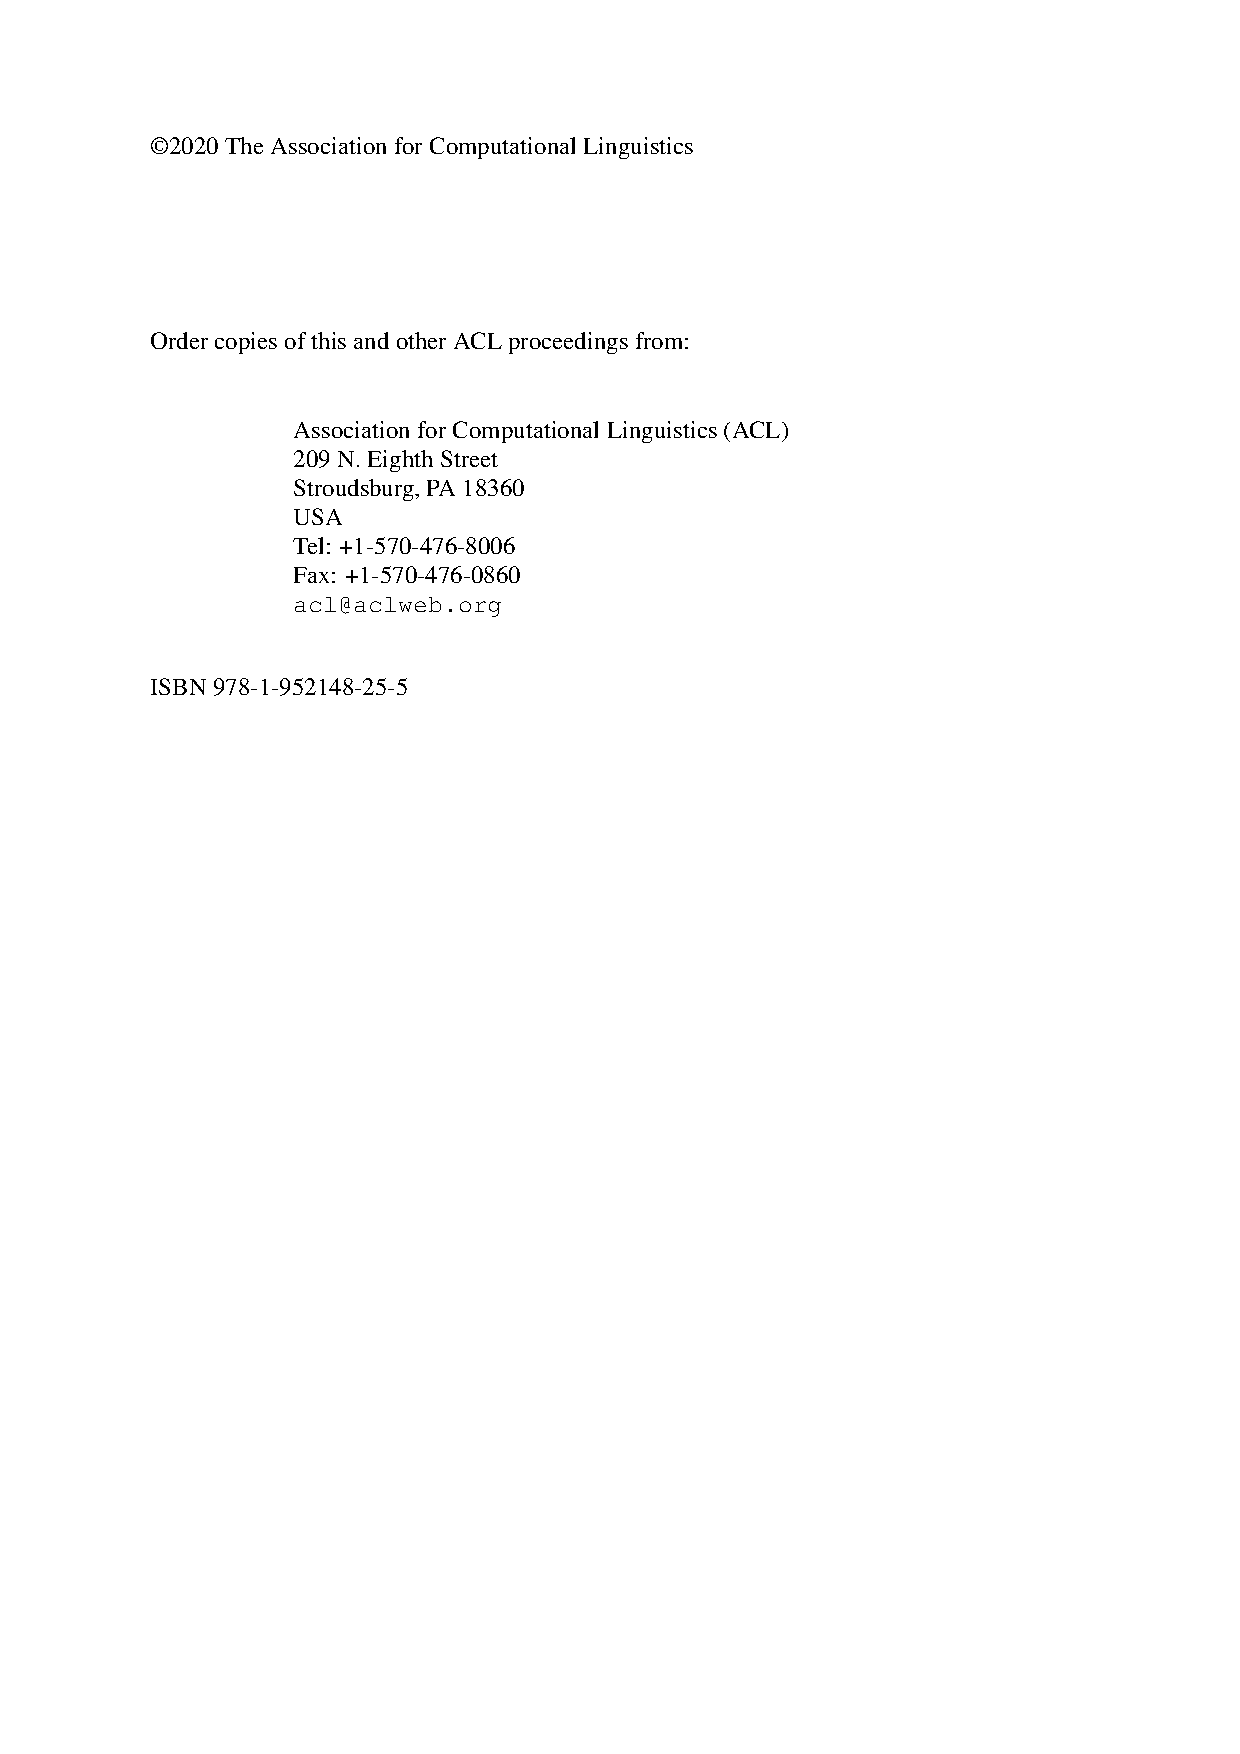
\includepdf{copyright.pdf}

\ifthenelse{\equal{\draftflag}{1}}{\draftframe}{}

\includepdf{preface.pdf}
%\ifthenelse{\isodd{\value{page}}}{}{\newpage \thispagestyle{empty} \phantom{.}}

\ifthenelse{\equal{\draftflag}{1}}{\draftframe}{}

\includepdf{organizers.pdf}
%\ifthenelse{\isodd{\value{page}}}{}{\newpage \thispagestyle{empty} \phantom{.}}

\ifthenelse{\equal{\draftflag}{1}}{\draftframe}{}
\setlength{\parindent}{0in}
\setlength{\parskip}{2ex}

\begin{center}
  {\Large \bf Table of Contents}
\end{center}

\vspace*{0.5cm}

\makeatletter
\renewcommand\tableofcontents{%
    \@starttoc{toc}%
}
\makeatother

\tableofcontents

%\ifthenelse{\isodd{\value{page}}}{}{\newpage \thispagestyle{empty} \phantom{.}}

%\ifthenelse{\equal{\draftflag}{1}}{\draftframe}{}
%\include{program}
%\ifthenelse{\isodd{\value{page}}}{}{\newpage \thispagestyle{empty} \phantom{.}}

% -------- INCLUDED PAPERS --------

\newpage
\pagenumbering{arabic}
\setcounter{page}{1}
\ClearShipoutPicture
\newcommand\invisiblesection[1]{%
  \refstepcounter{section}%
  \addcontentsline{toc}{section}{#1}%
  \sectionmark{#1}}

\refstepcounter{chapter}
\addcontentsline{toc}{chapter}{Full Papers}
\sectionmark{Full Papers}

\invisiblesection{Nataly Jahchan, Anne Condamines, Emmanuelle Cannesson and Helene Giraudo. Towards a More Natural Controlled Language in Future Airbus Cockpits. A Psycho-linguistic Evaluation}
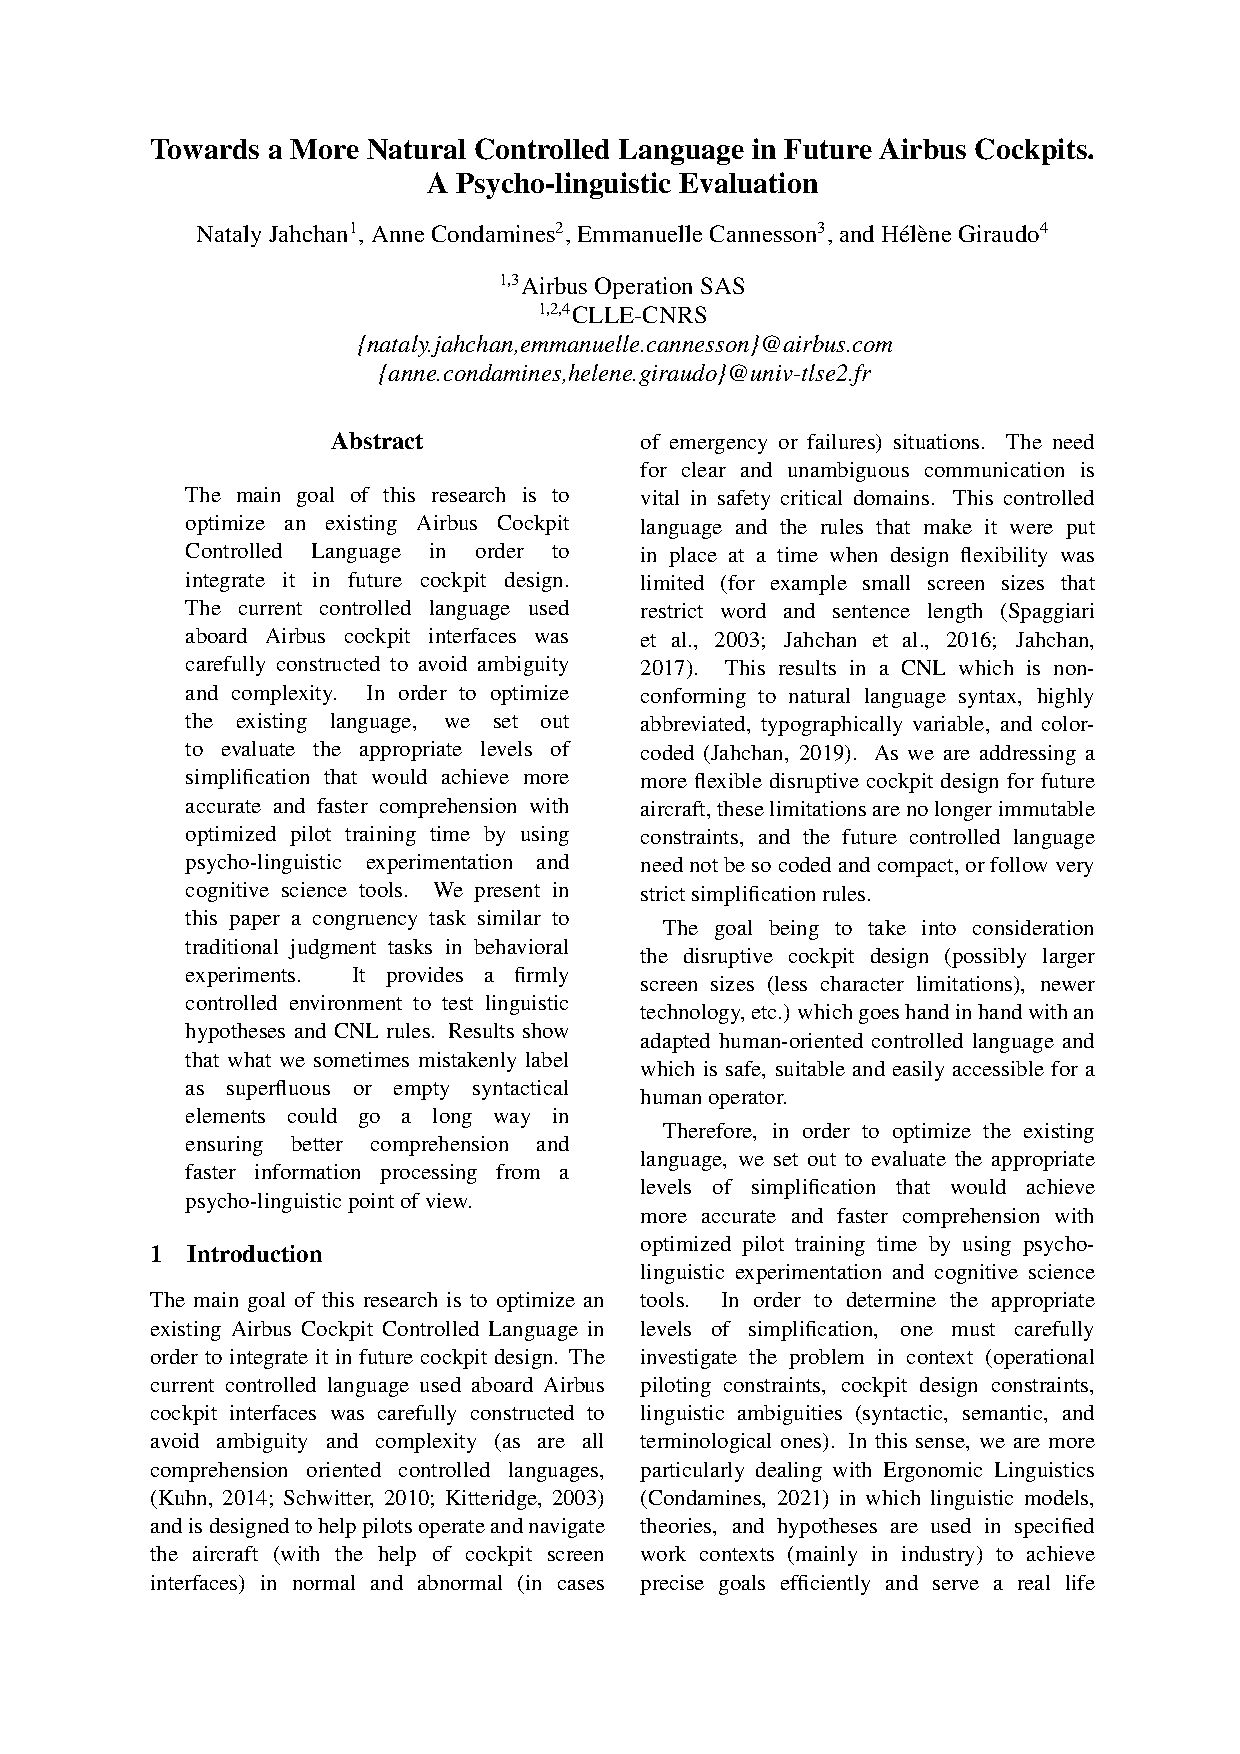
\includepdf[pages=-,pagecommand={}]{../cdrom/pdf/2021.cnl-1.1.pdf}

\invisiblesection{Arianna Masciolini and Aarne Ranta. Grammar-Based Concept Alignment for Domain-Specific Machine Translation}
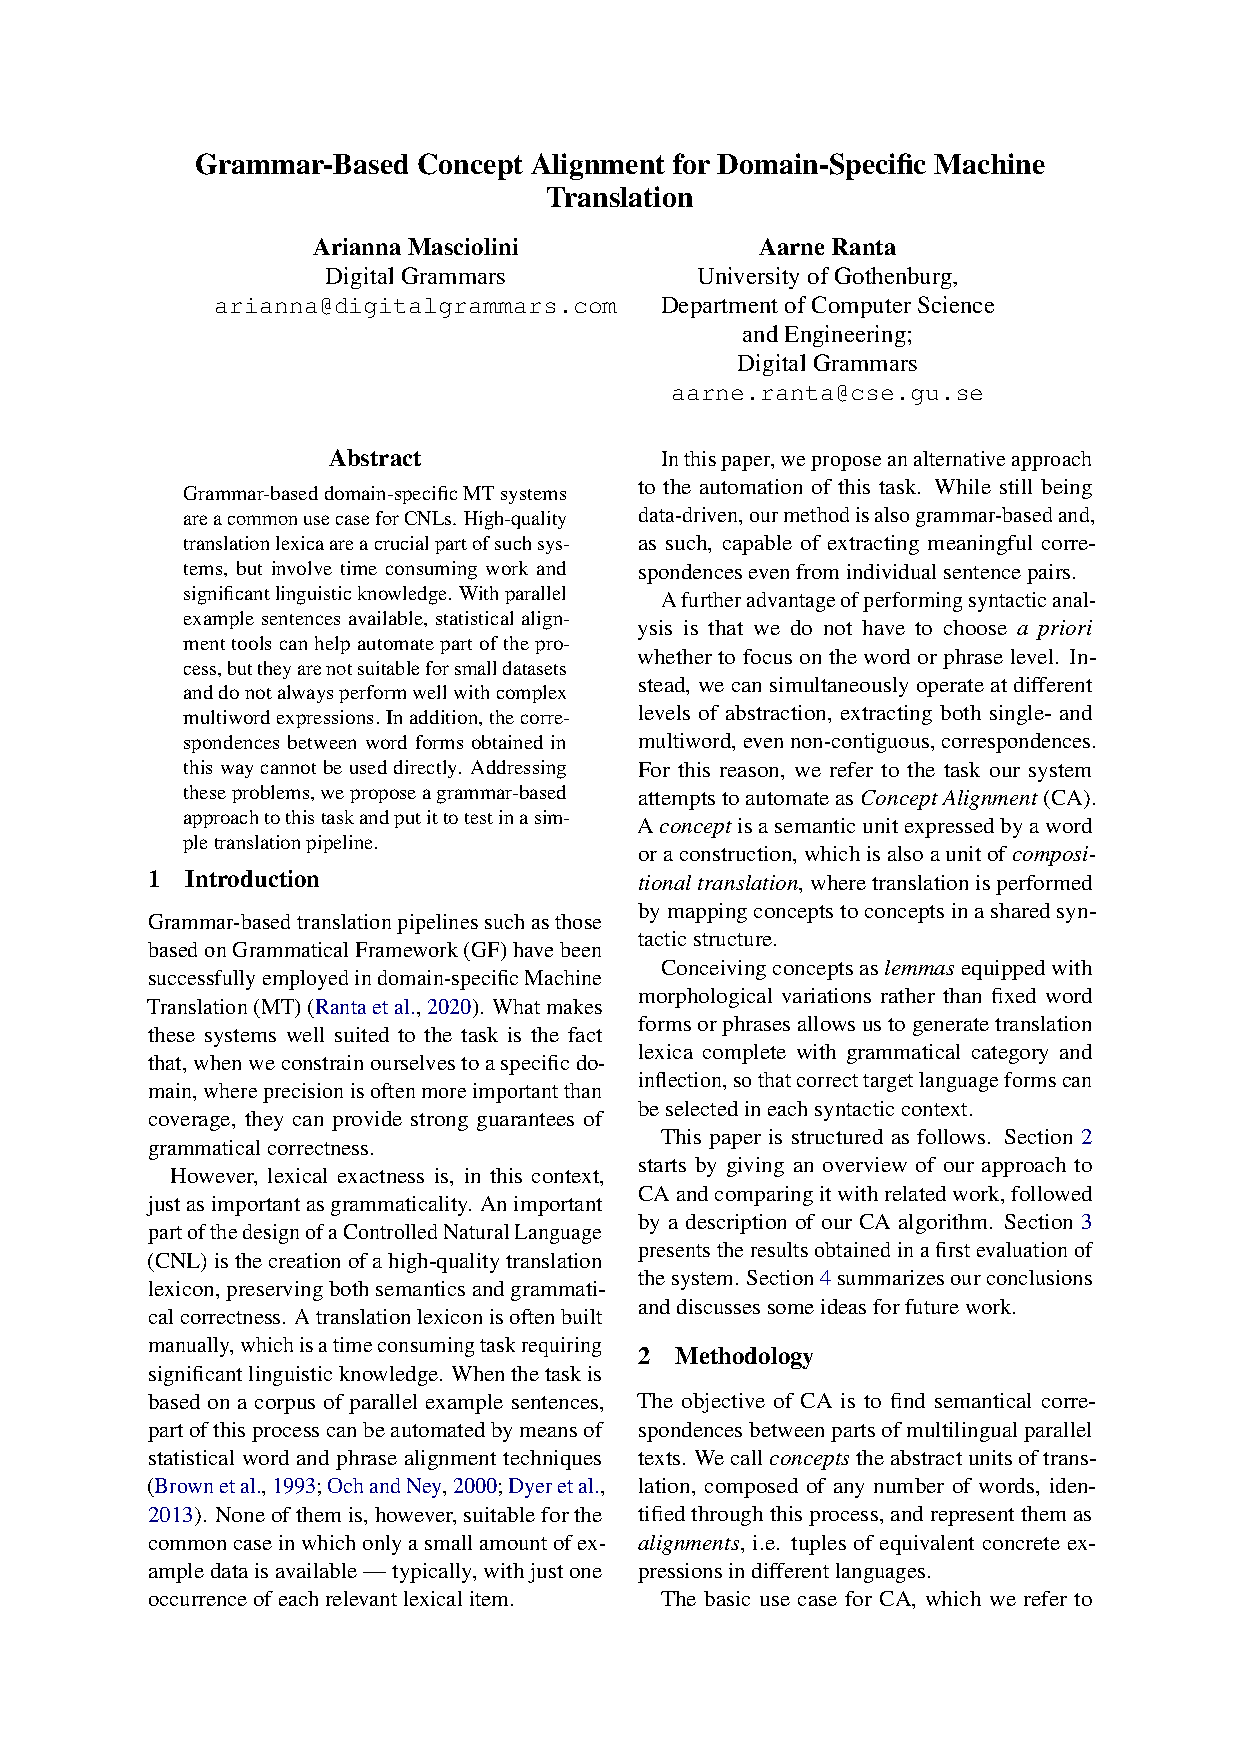
\includepdf[pages=-,pagecommand={}]{../cdrom/pdf/2021.cnl-1.2.pdf}

\invisiblesection{TODO}
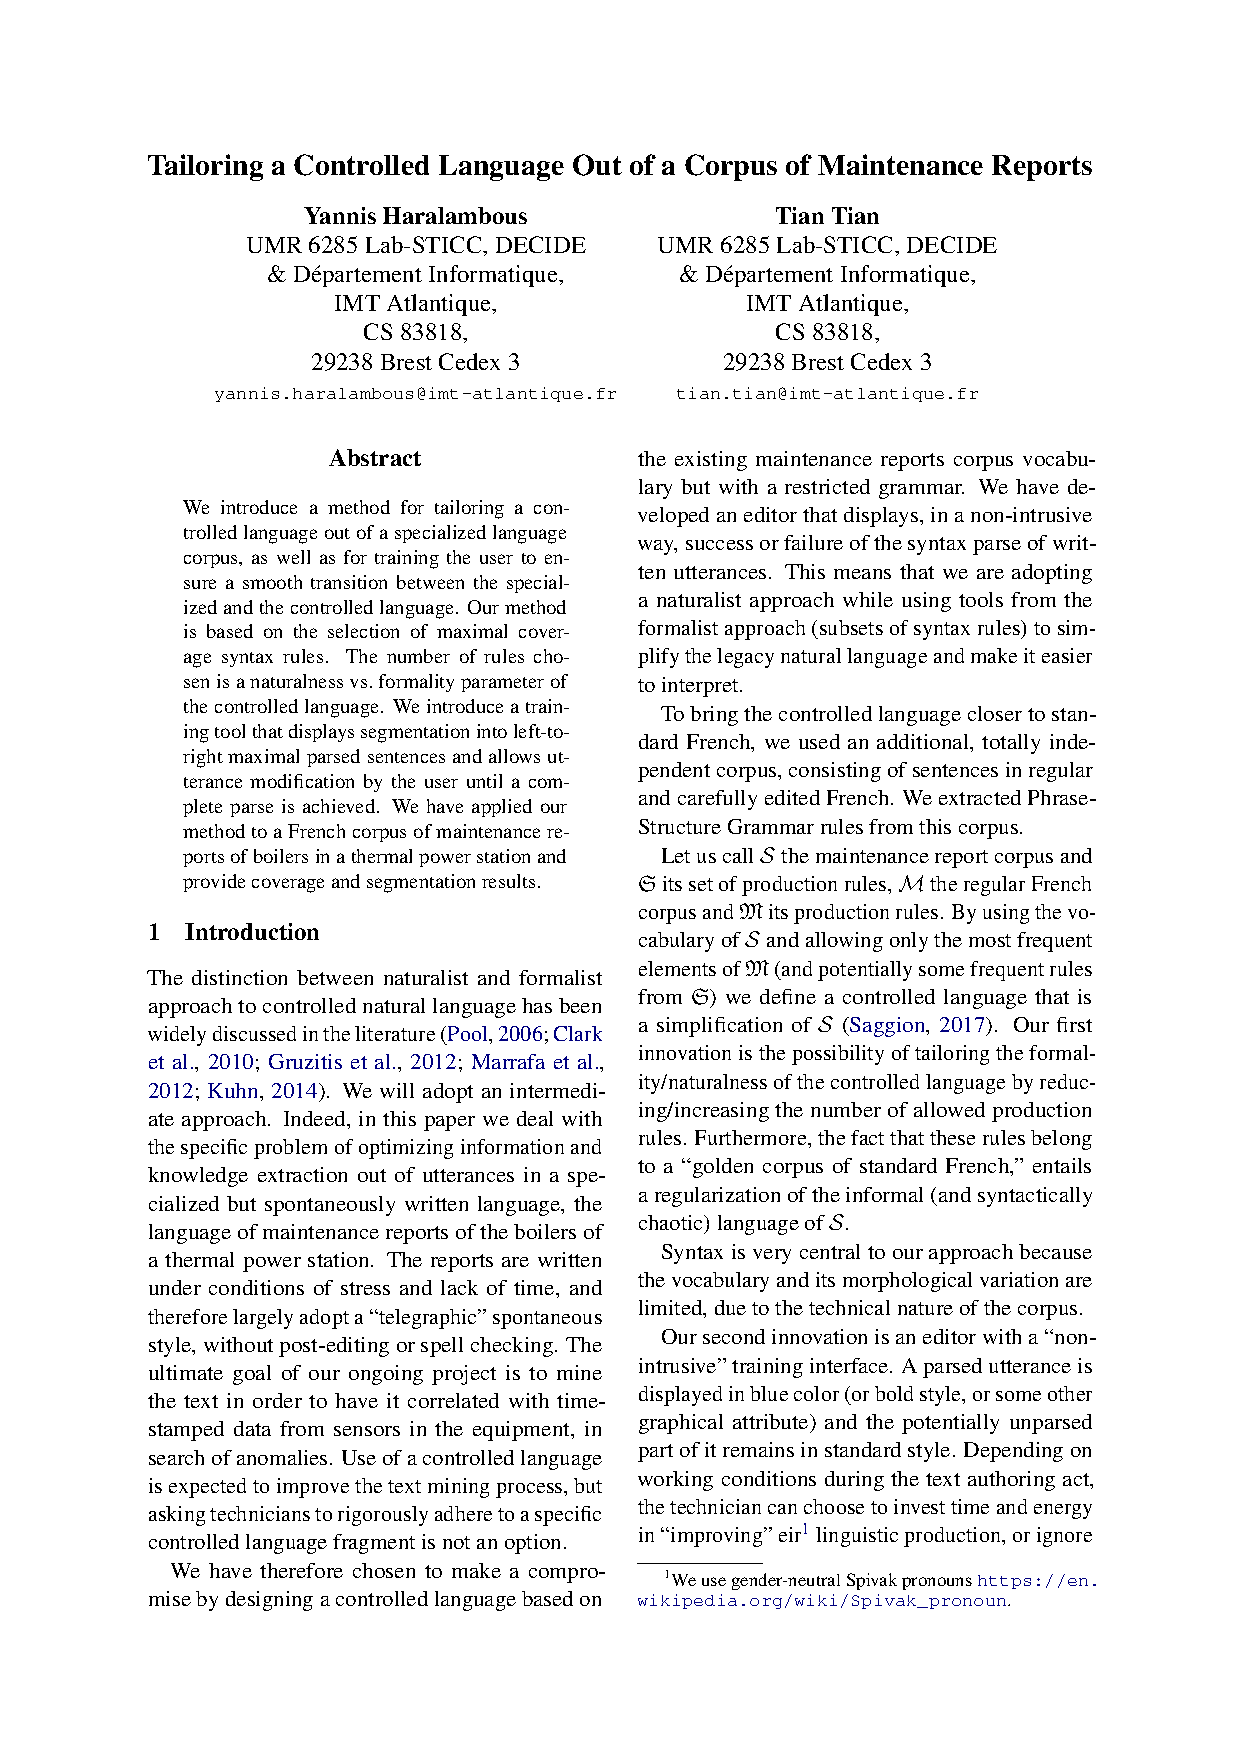
\includepdf[pages=-,pagecommand={}]{../cdrom/pdf/2021.cnl-1.3.pdf}

\invisiblesection{TODO}
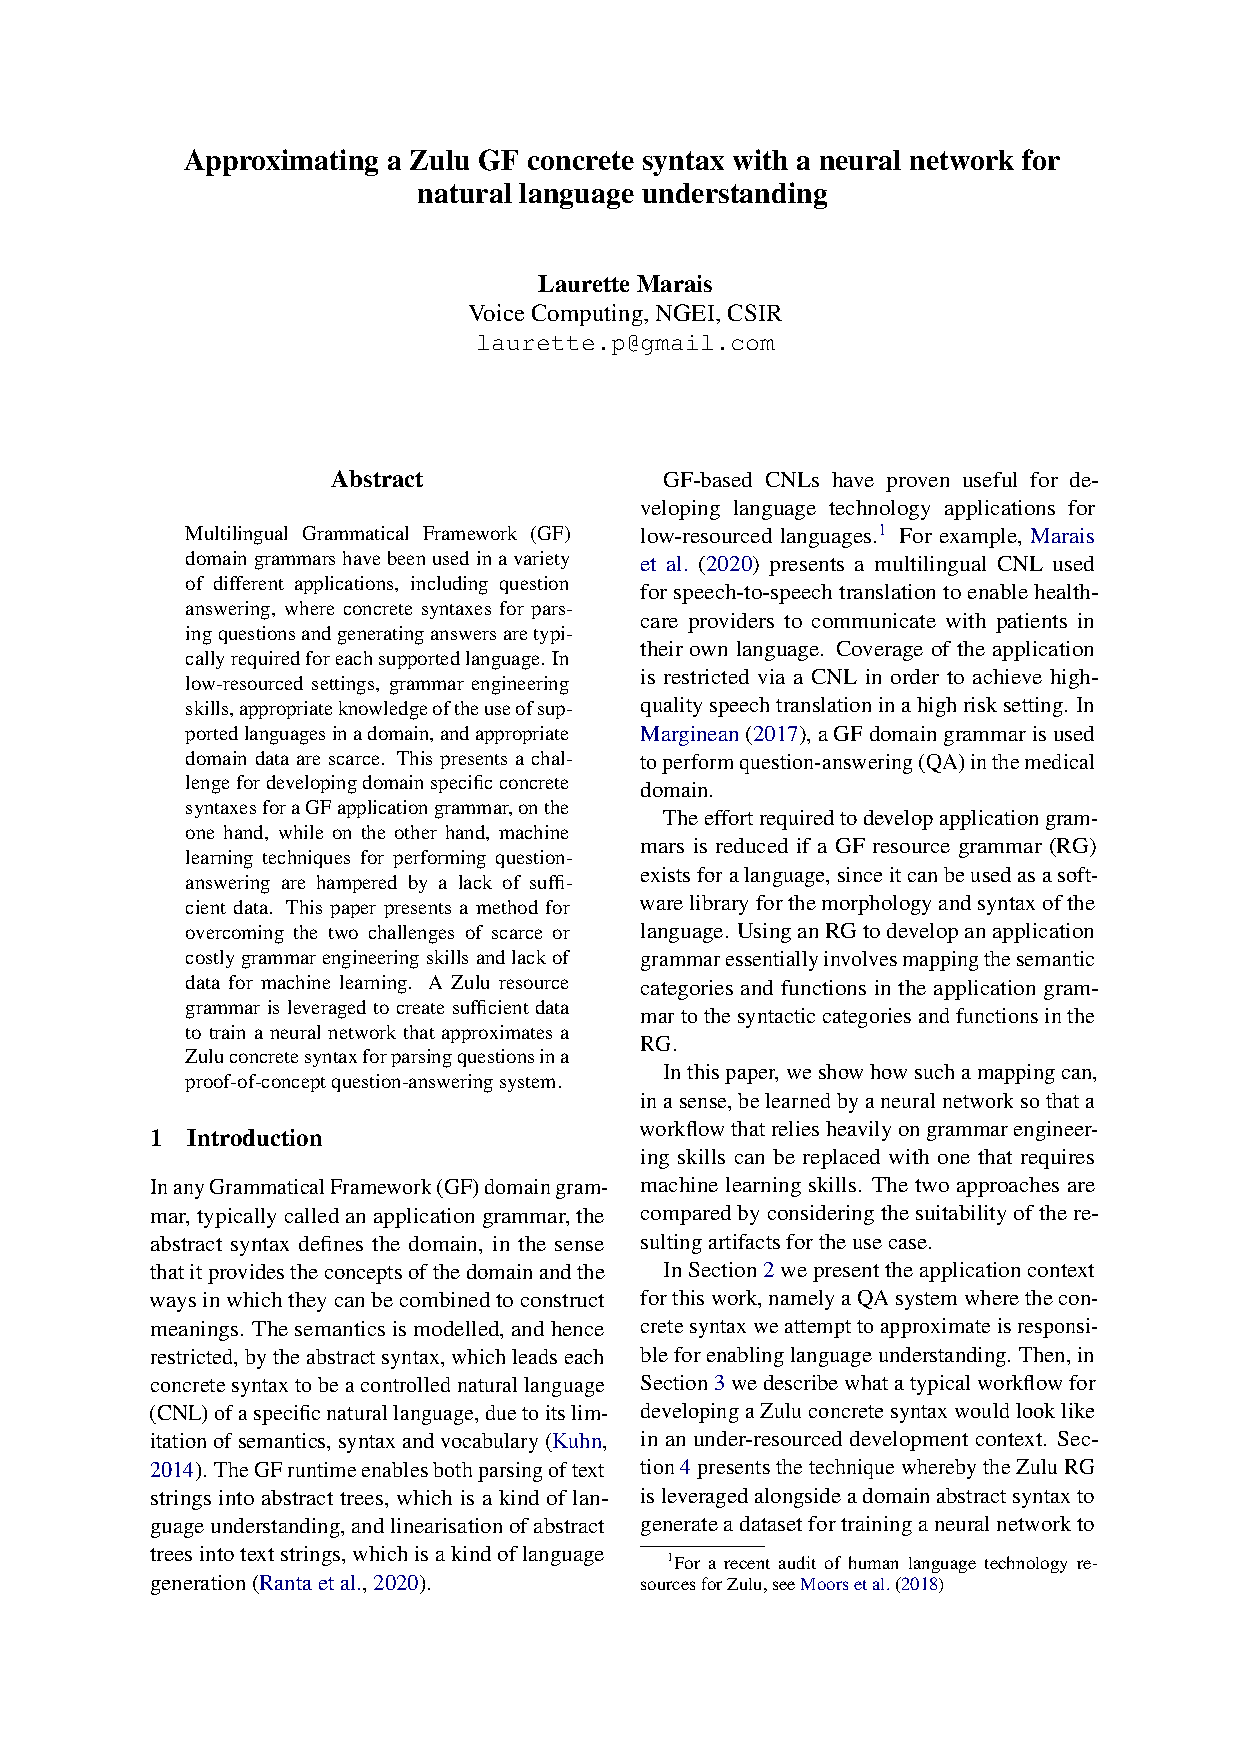
\includepdf[pages=-,pagecommand={}]{../cdrom/pdf/2021.cnl-1.4.pdf}

\invisiblesection{TODO}
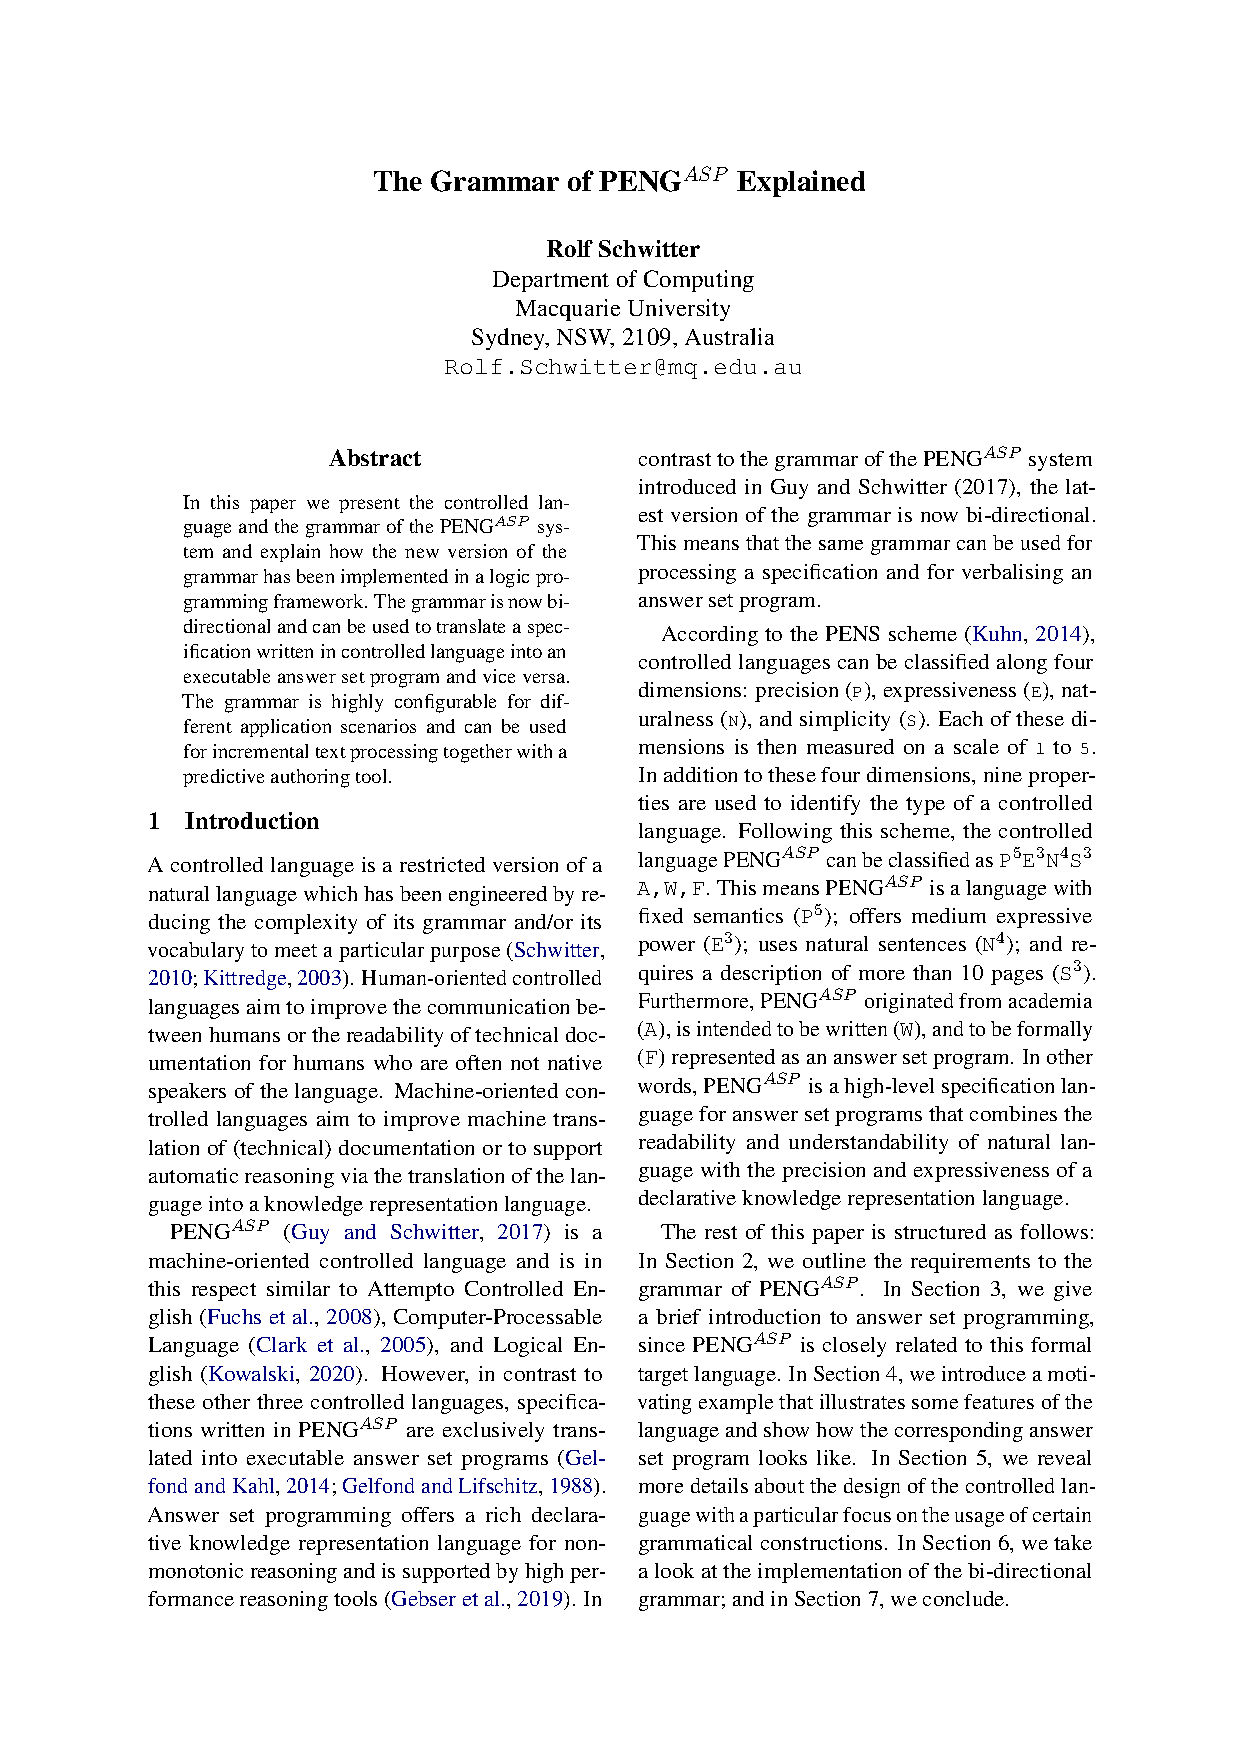
\includepdf[pages=-,pagecommand={}]{../cdrom/pdf/2021.cnl-1.5.pdf}

\invisiblesection{TODO}
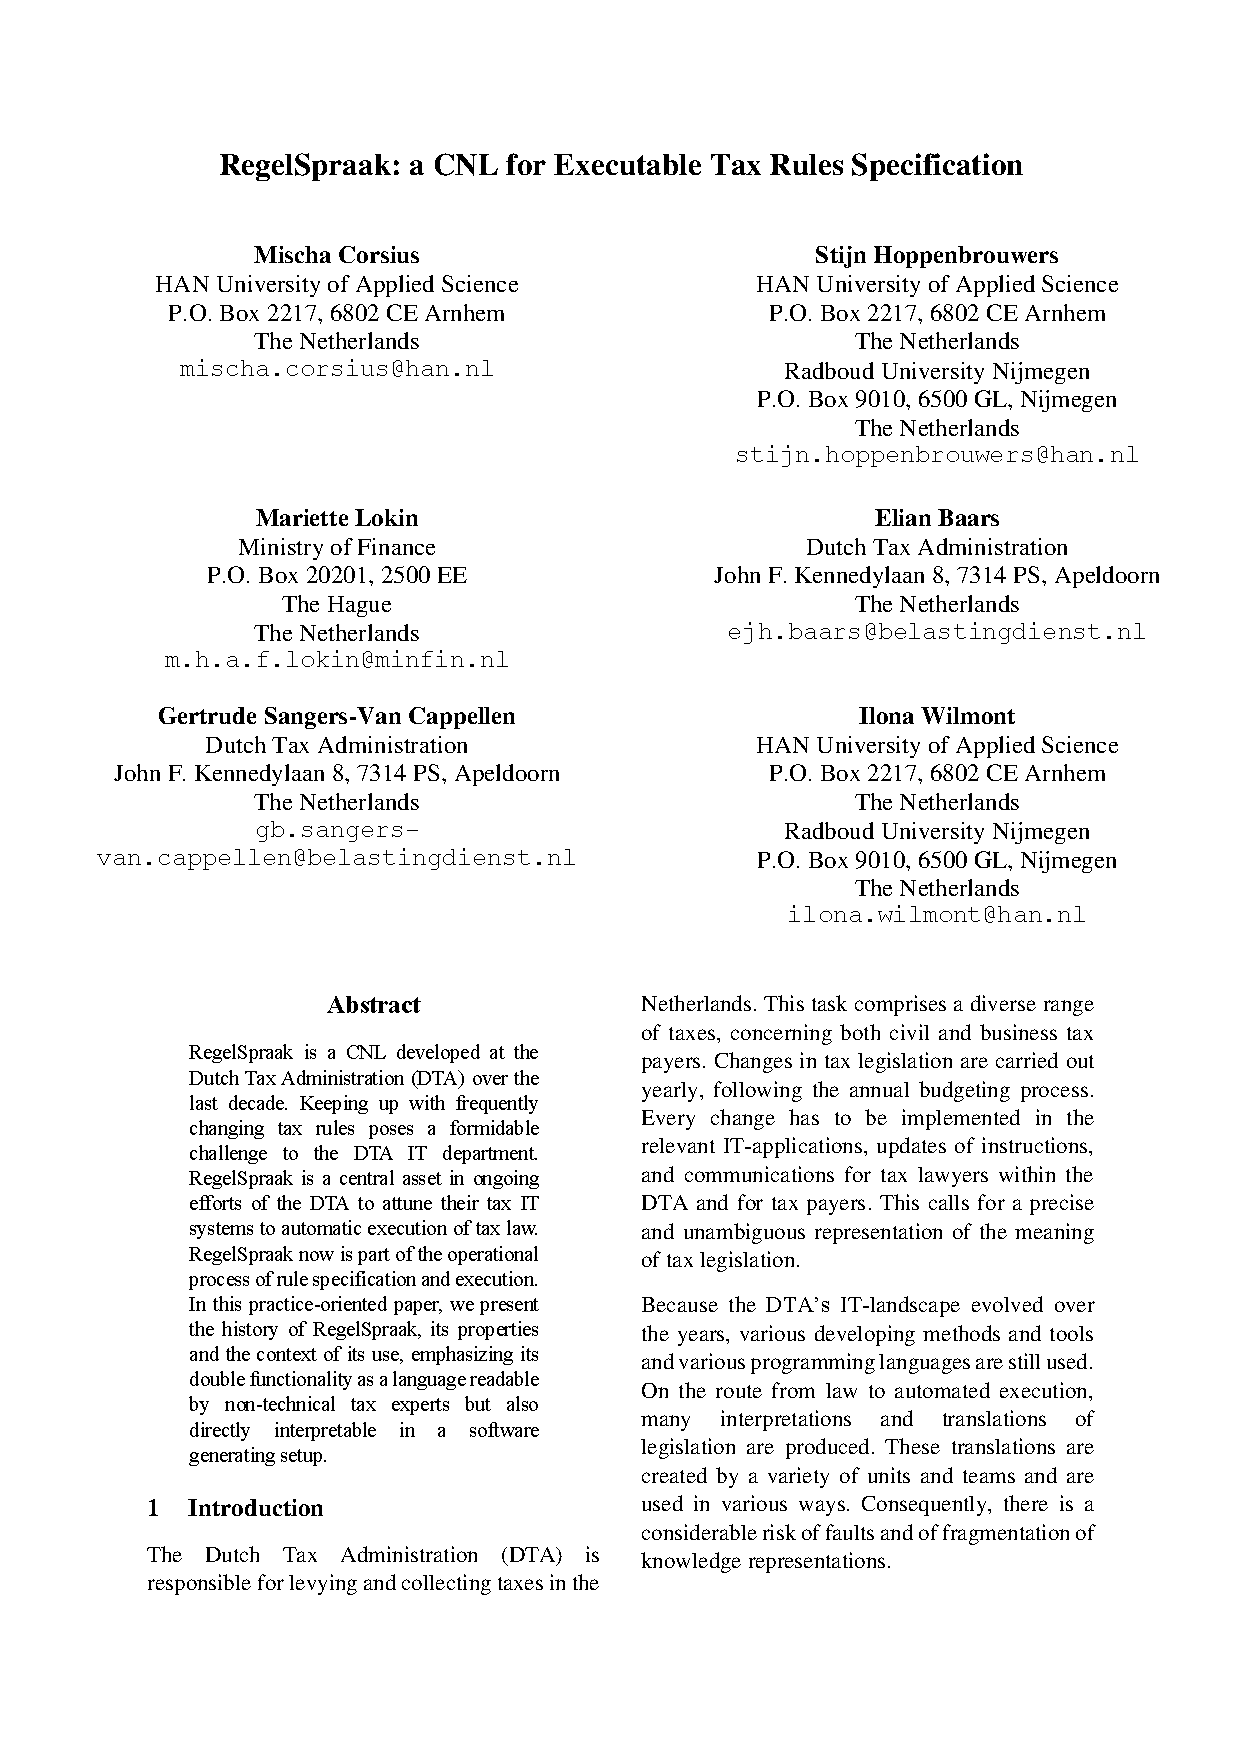
\includepdf[pages=-,pagecommand={}]{../cdrom/pdf/2021.cnl-1.6.pdf}

\invisiblesection{TODO}
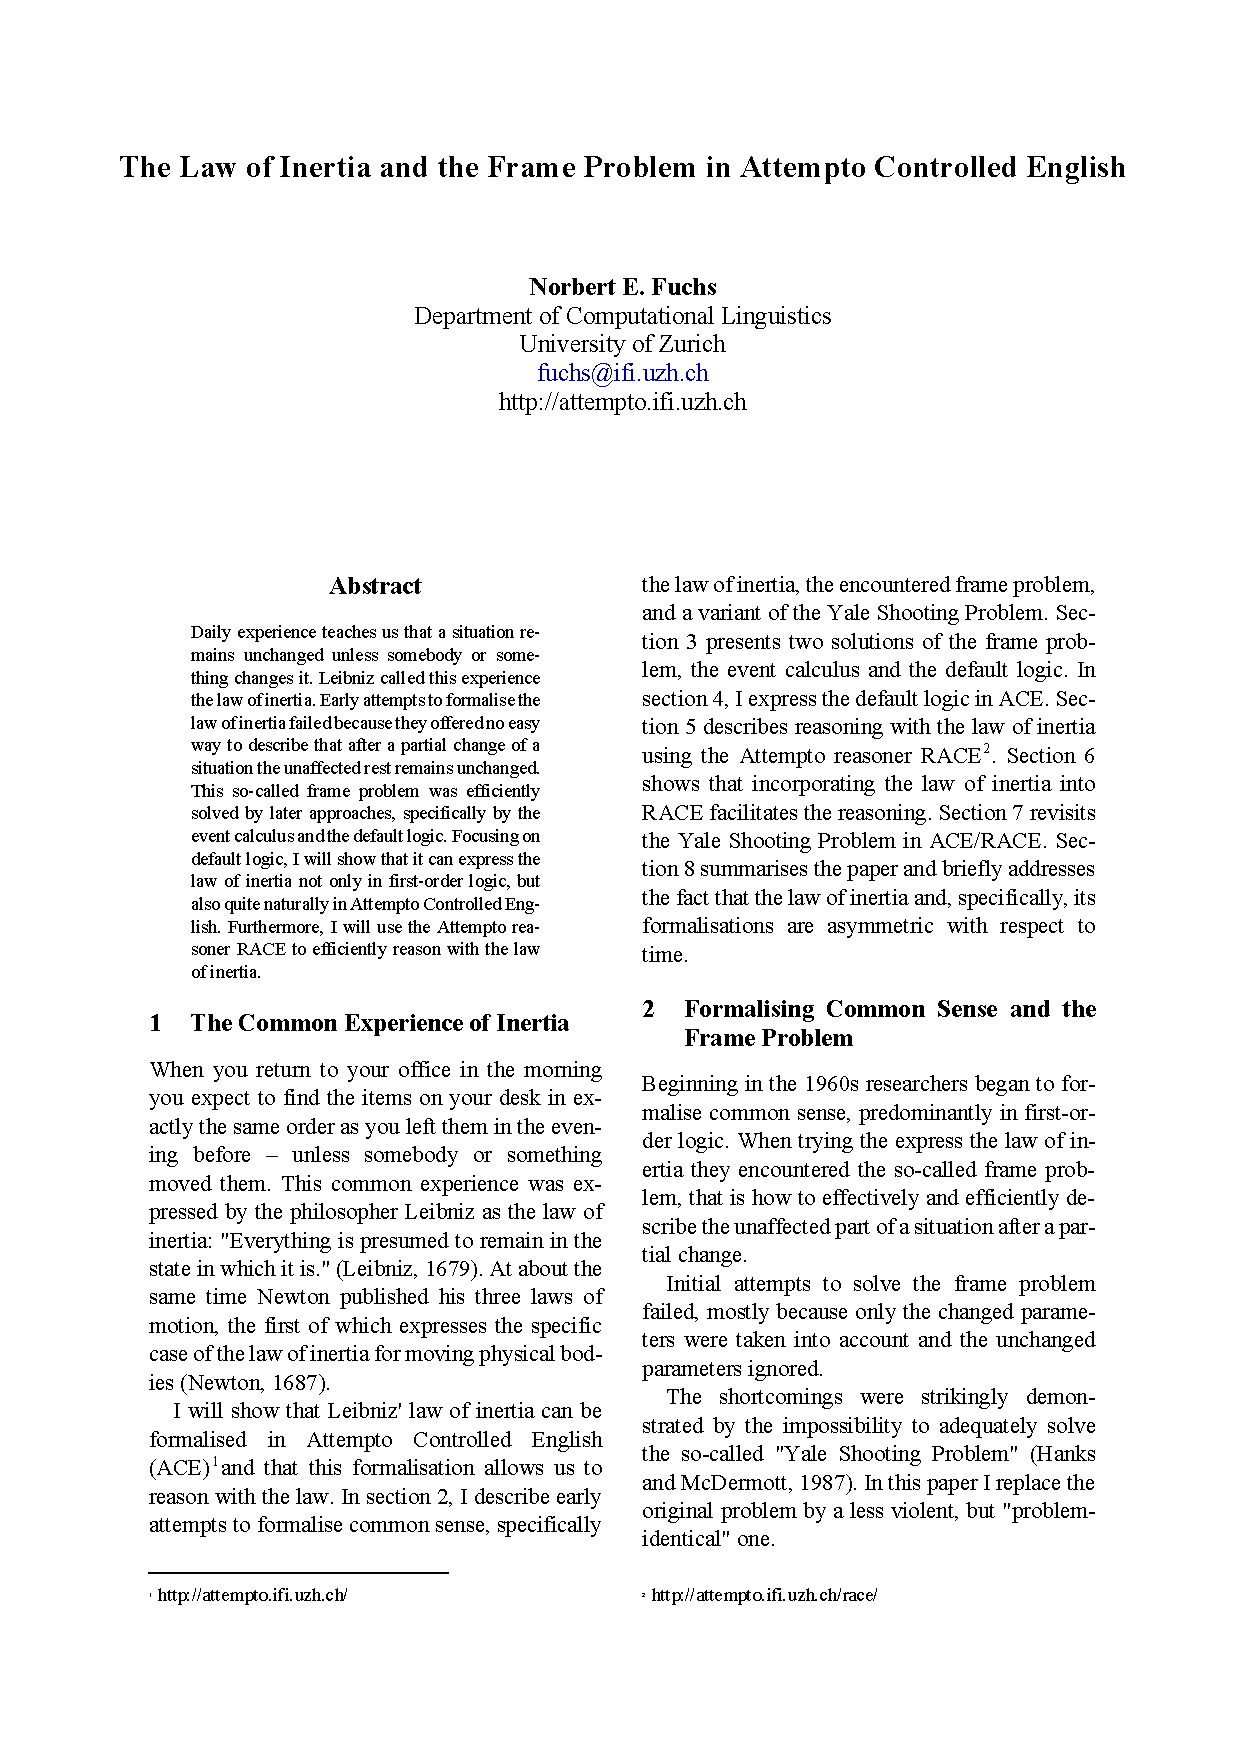
\includepdf[pages=-,pagecommand={}]{../cdrom/pdf/2021.cnl-1.7.pdf}

\invisiblesection{TODO}
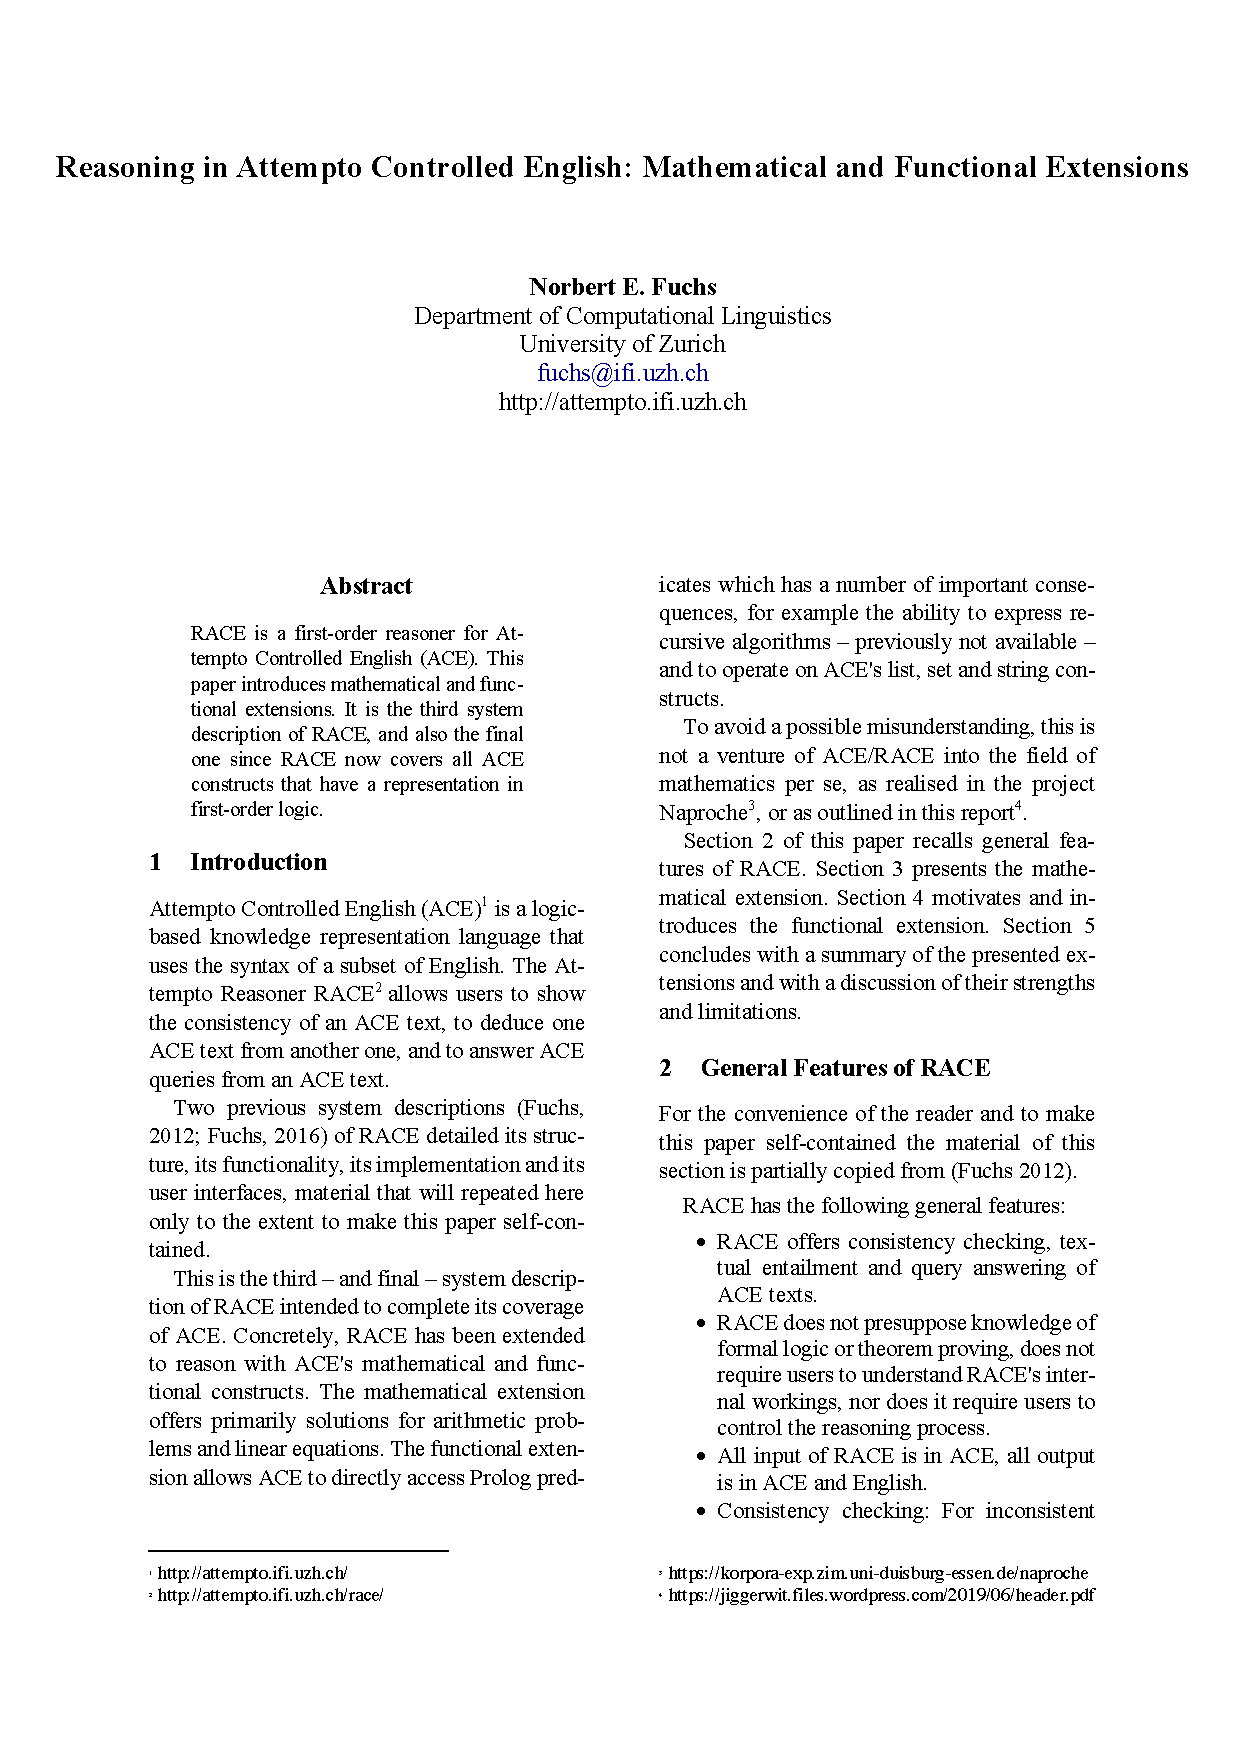
\includepdf[pages=-,pagecommand={}]{../cdrom/pdf/2021.cnl-1.8.pdf}

\invisiblesection{TODO}
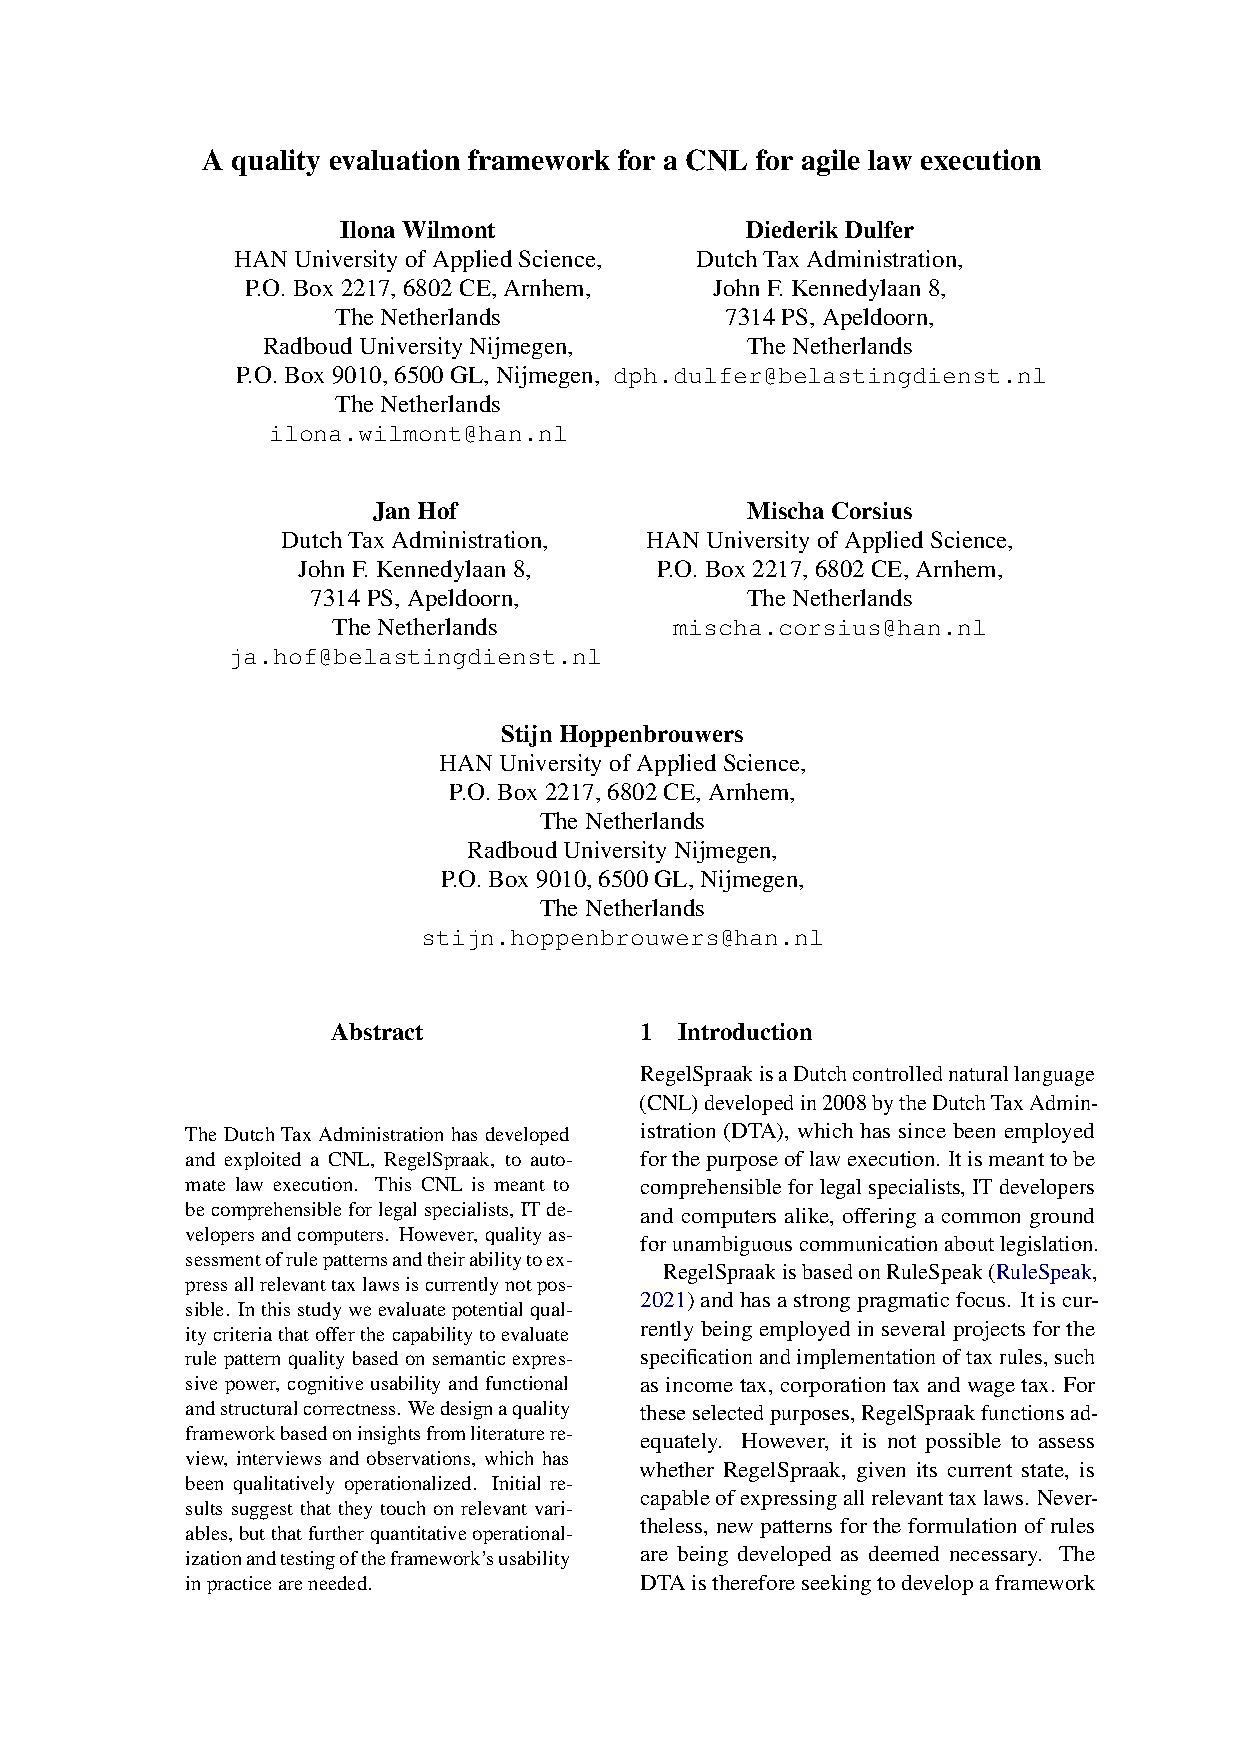
\includepdf[pages=-,pagecommand={}]{../cdrom/pdf/2021.cnl-1.9.pdf}

\invisiblesection{TODO}
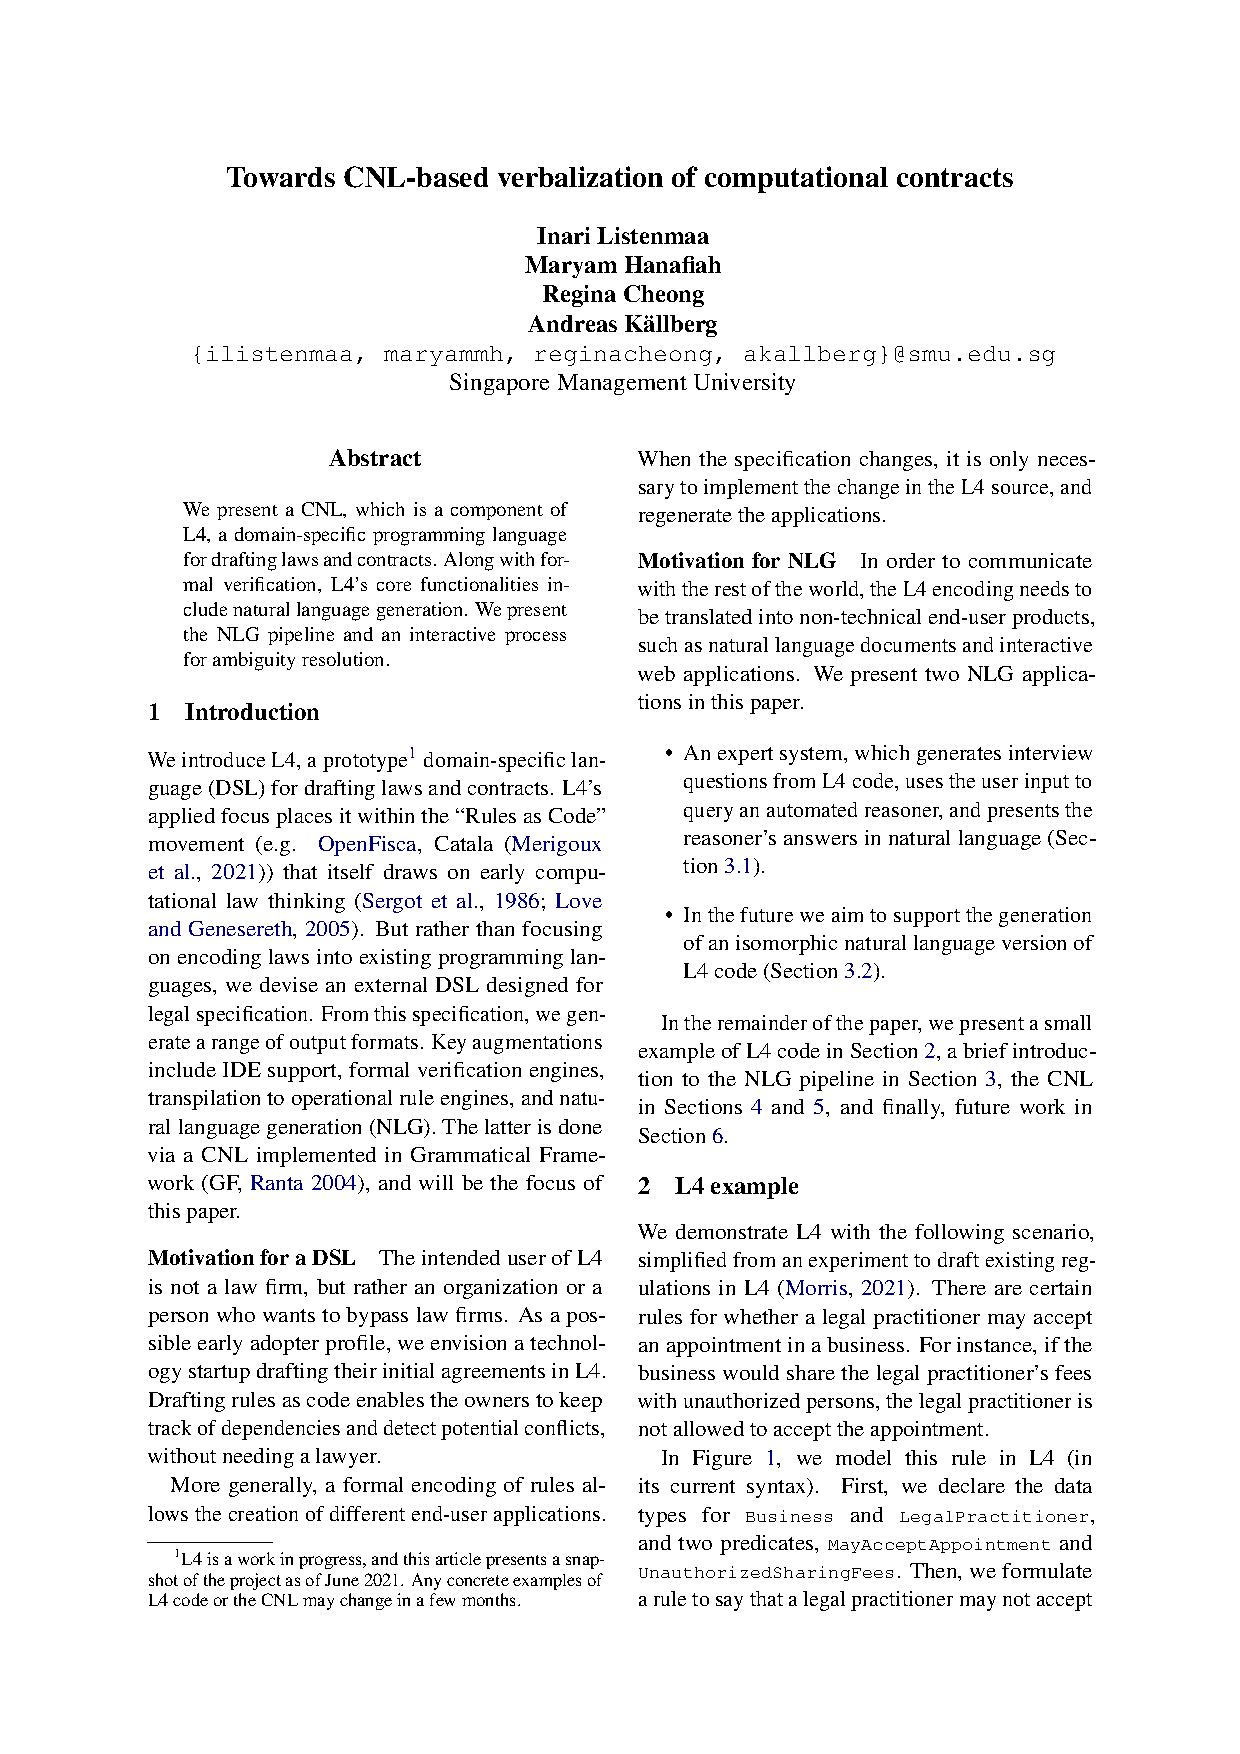
\includepdf[pages=-,pagecommand={}]{../cdrom/pdf/2021.cnl-1.10.pdf}

\invisiblesection{TODO}
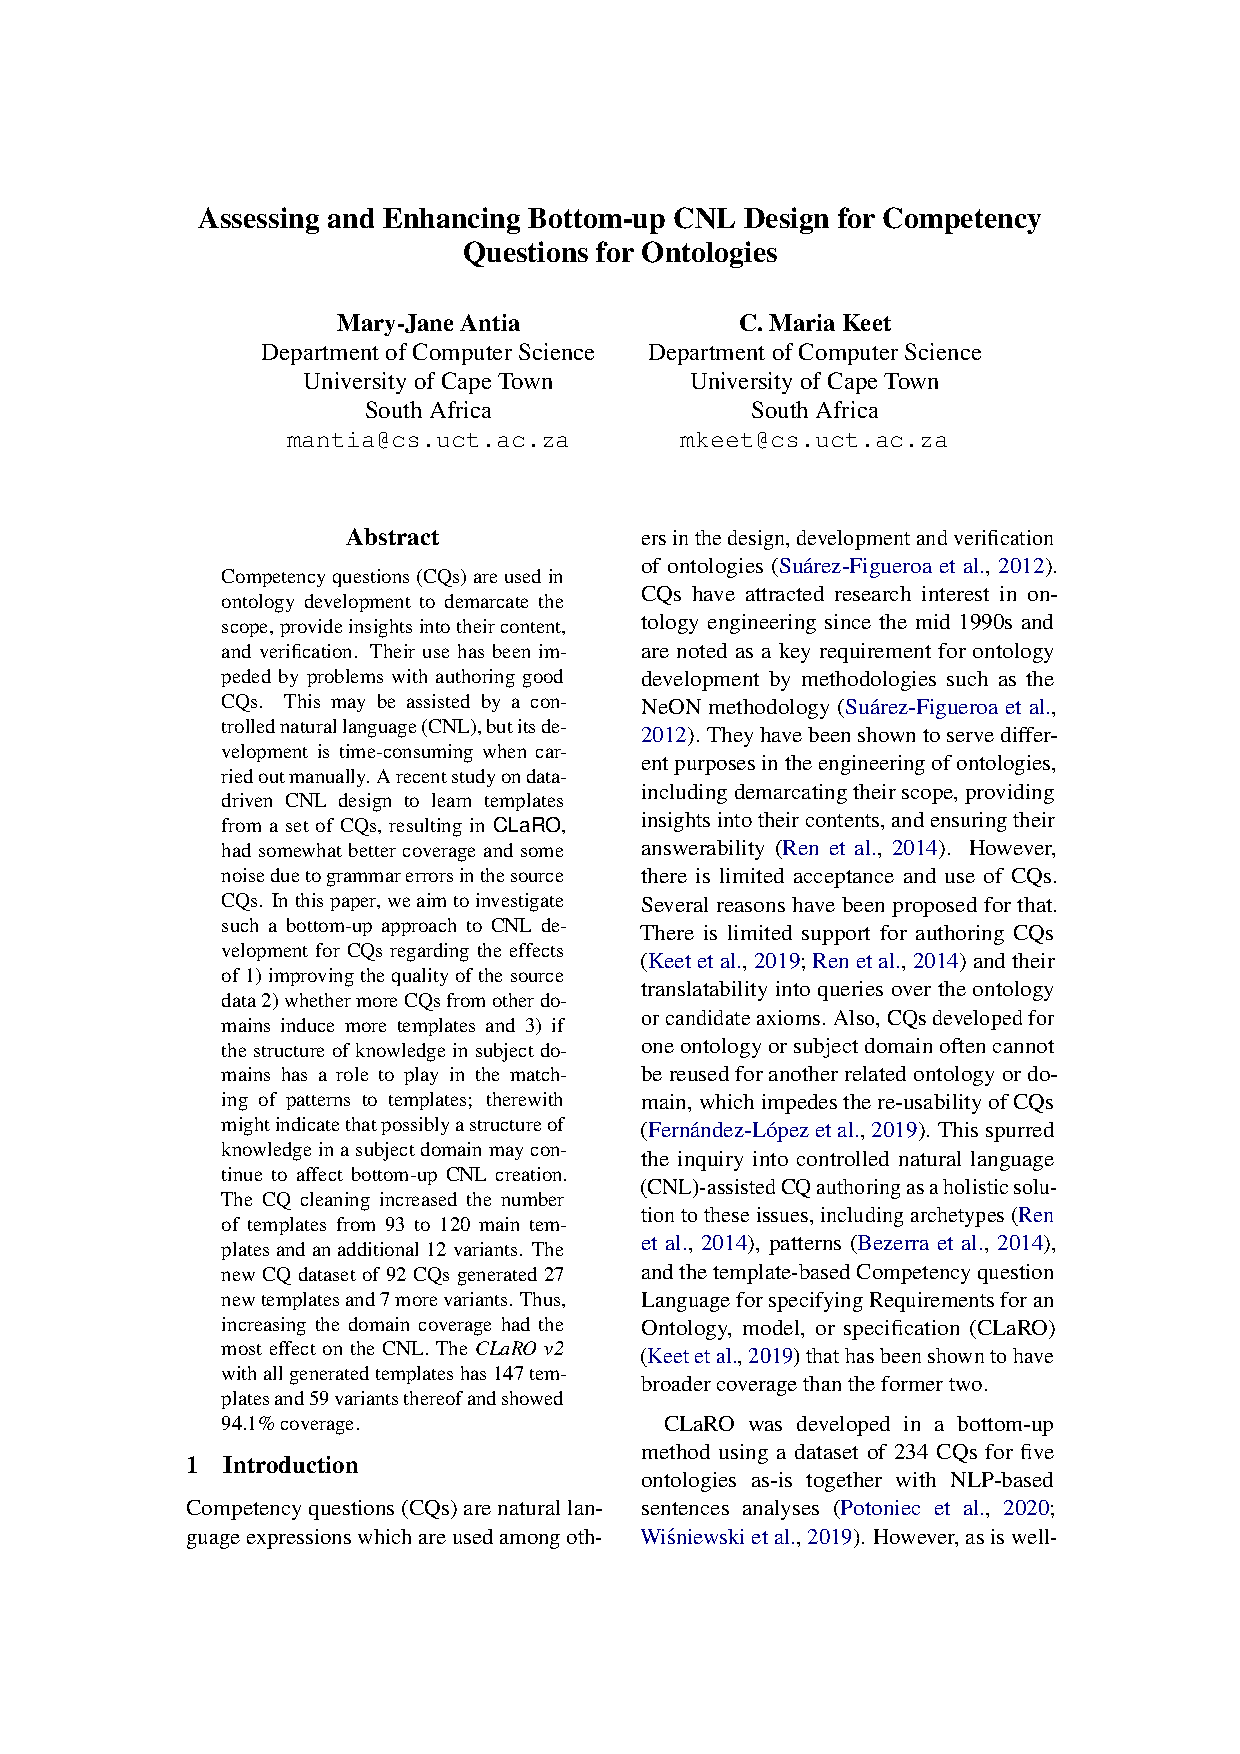
\includepdf[pages=-,pagecommand={}]{../cdrom/pdf/2021.cnl-1.11.pdf}


\refstepcounter{chapter}
\addcontentsline{toc}{chapter}{Short Papers}
\sectionmark{Short Papers}

\invisiblesection{TODO}
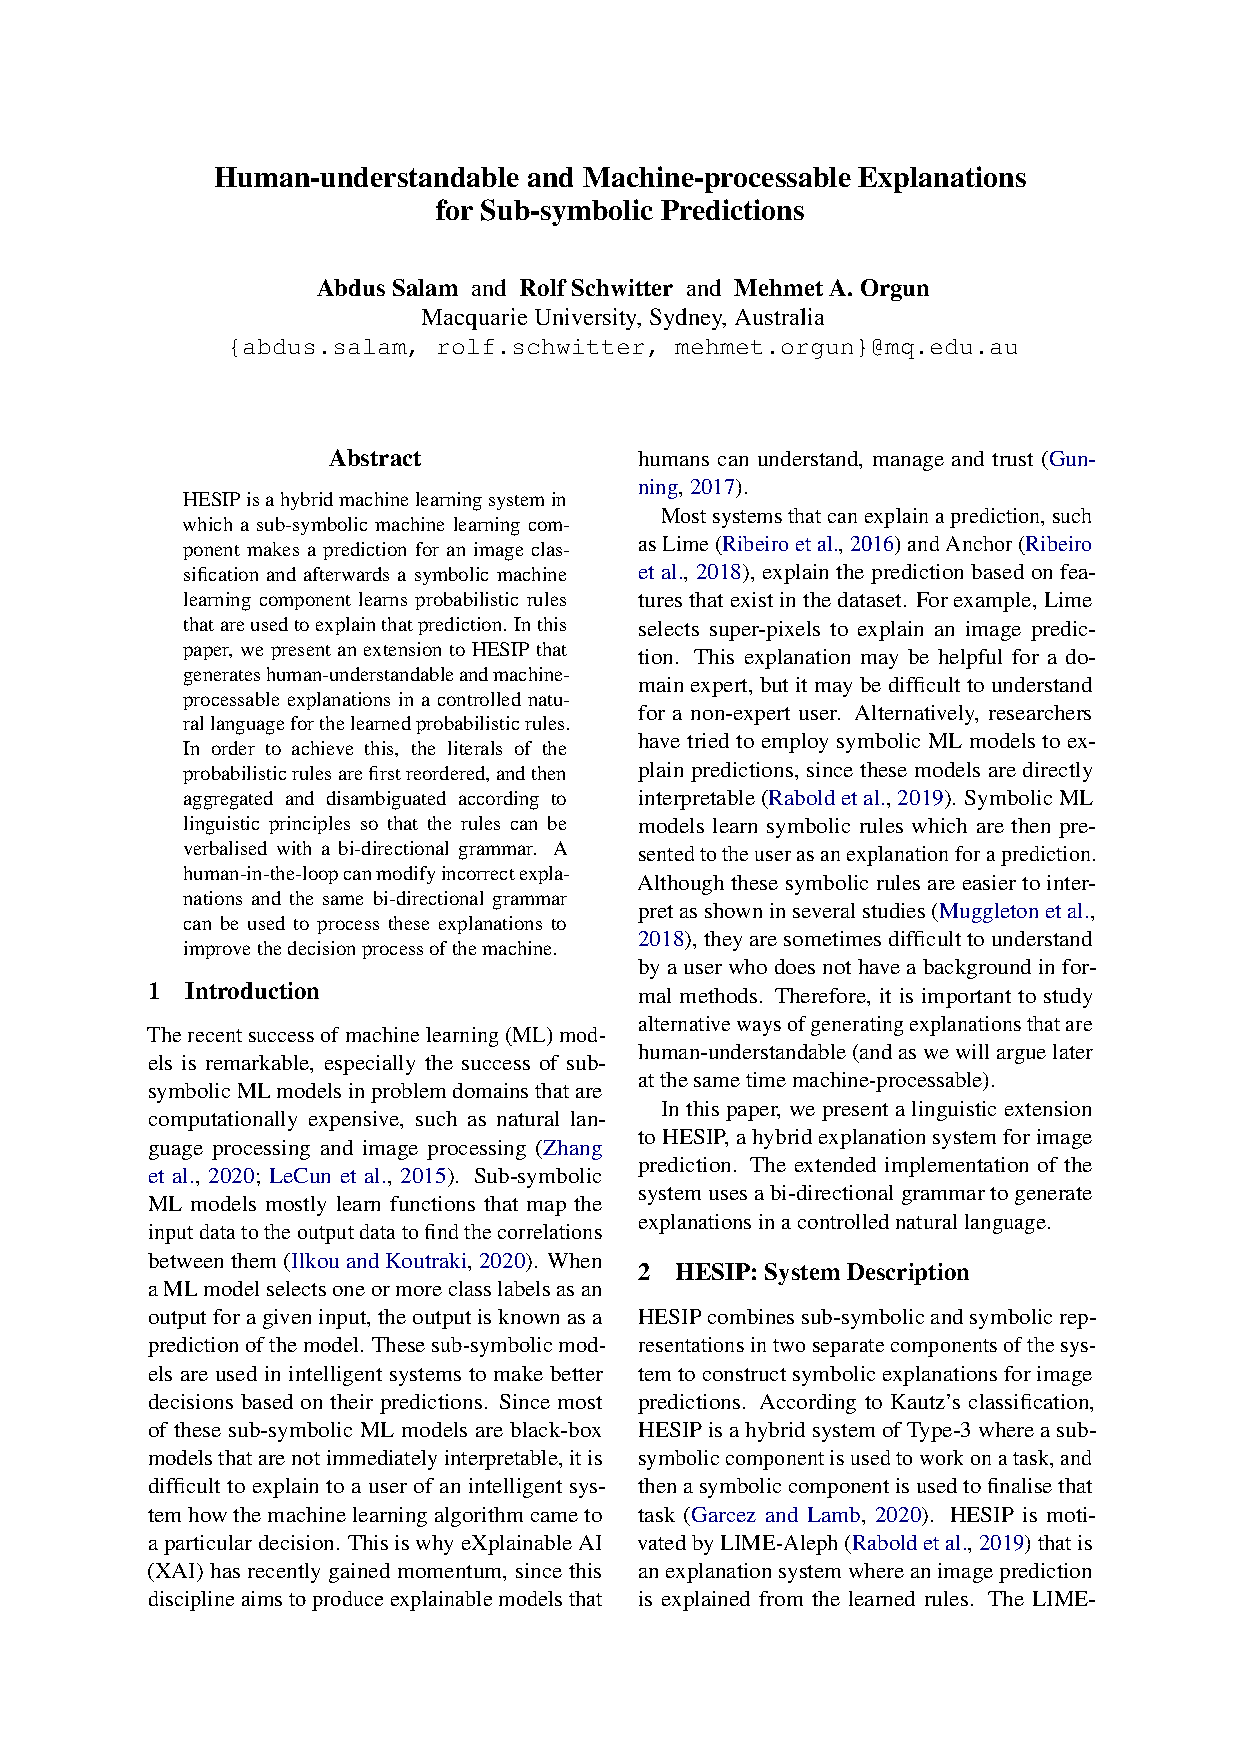
\includepdf[pages=-,pagecommand={}]{../cdrom/pdf/2021.cnl-1.12.pdf}

\invisiblesection{TODO}
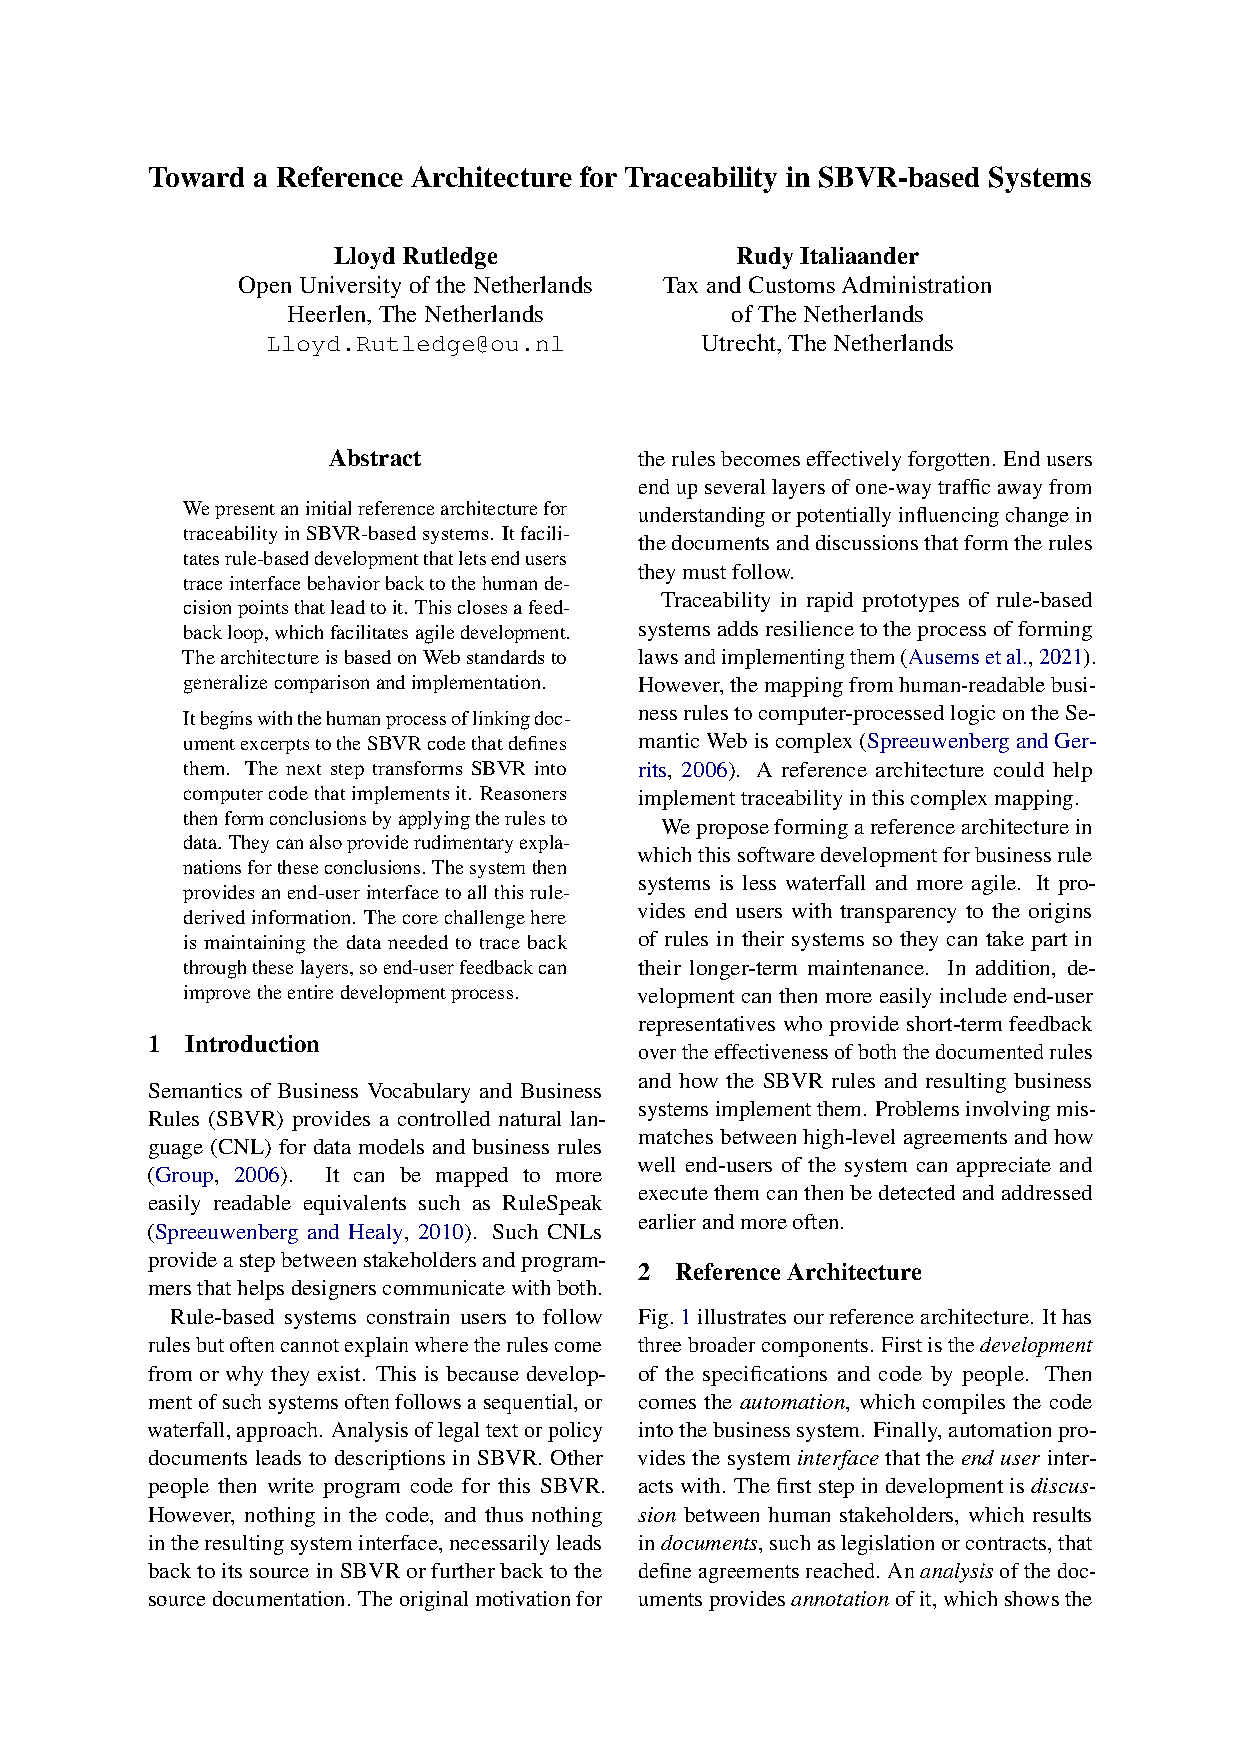
\includepdf[pages=-,pagecommand={}]{../cdrom/pdf/2021.cnl-1.13.pdf}

\invisiblesection{TODO}
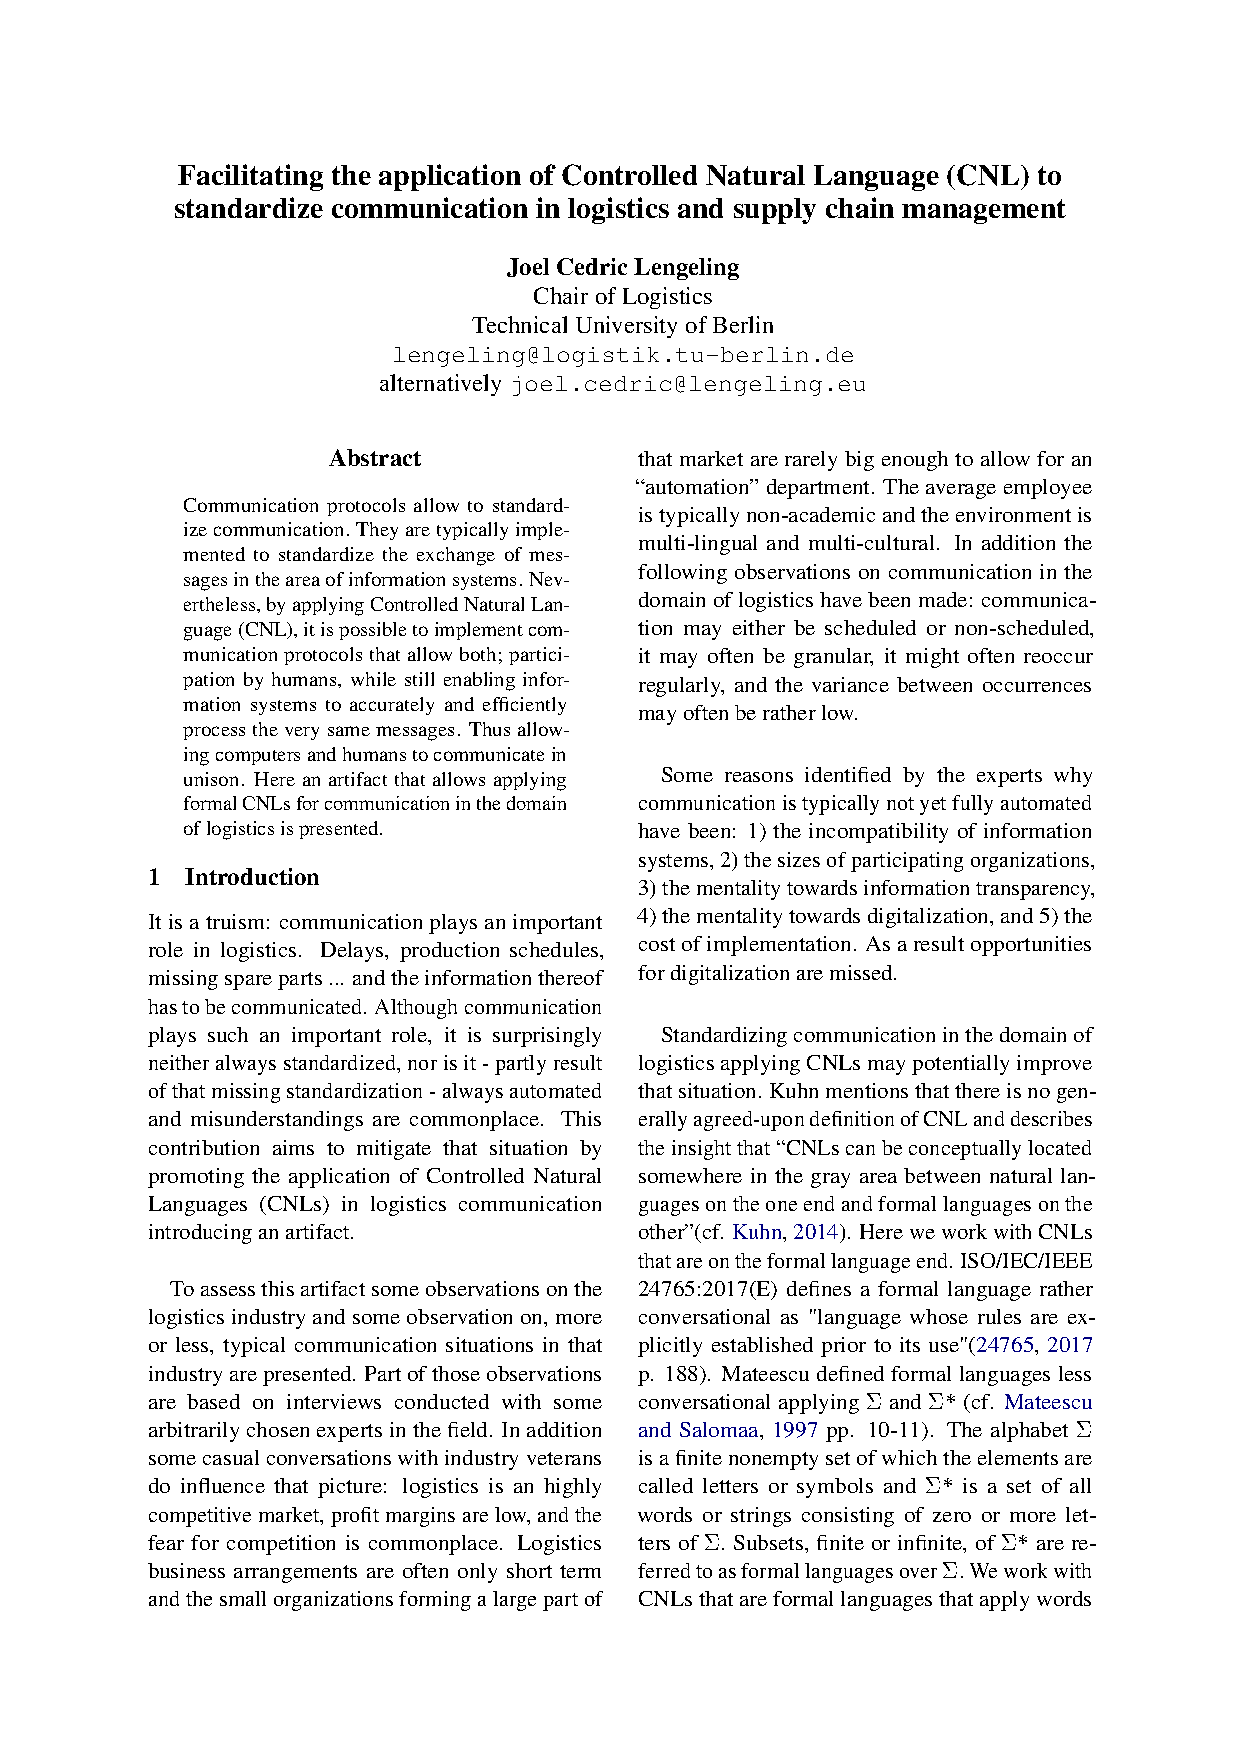
\includepdf[pages=-,pagecommand={}]{../cdrom/pdf/2021.cnl-1.14.pdf}

\invisiblesection{TODO}
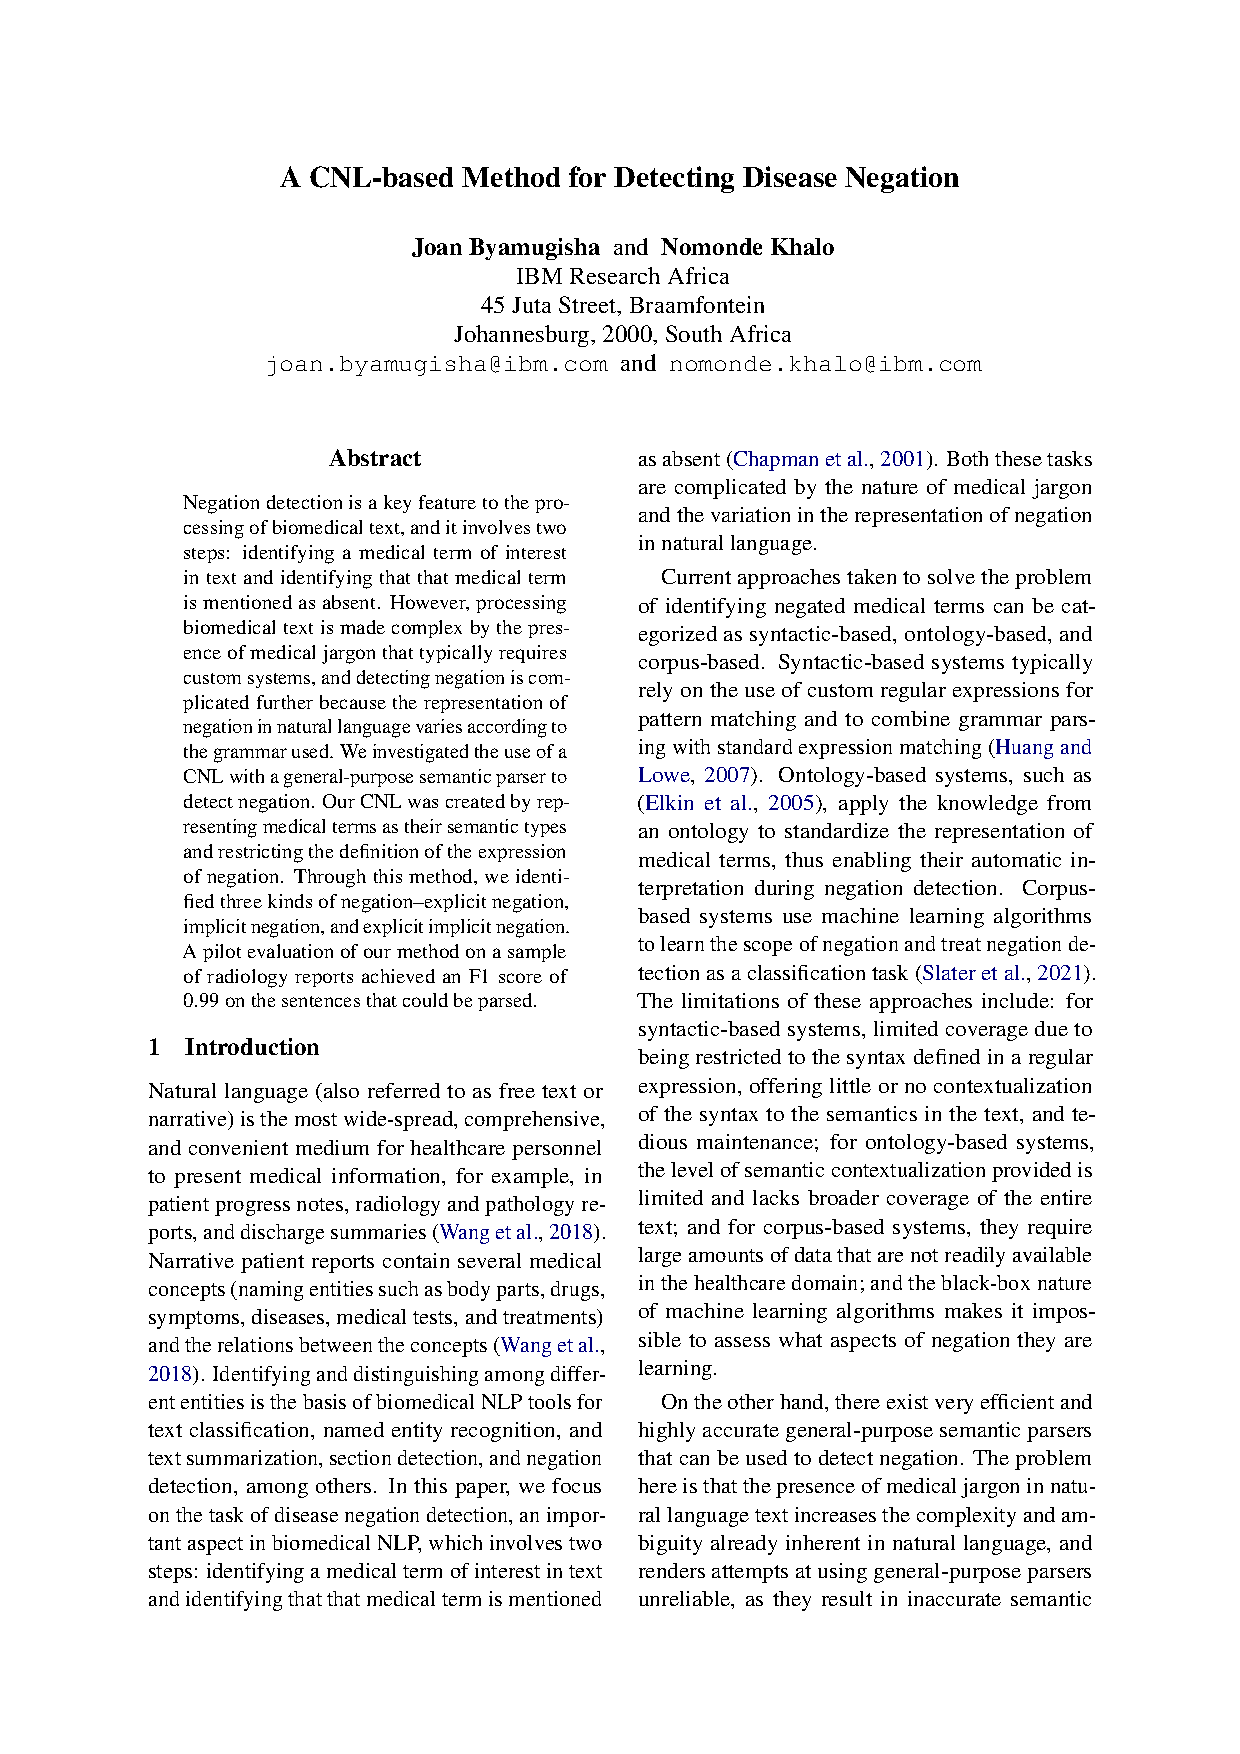
\includepdf[pages=-,pagecommand={}]{../cdrom/pdf/2021.cnl-1.15.pdf}

\invisiblesection{TODO}
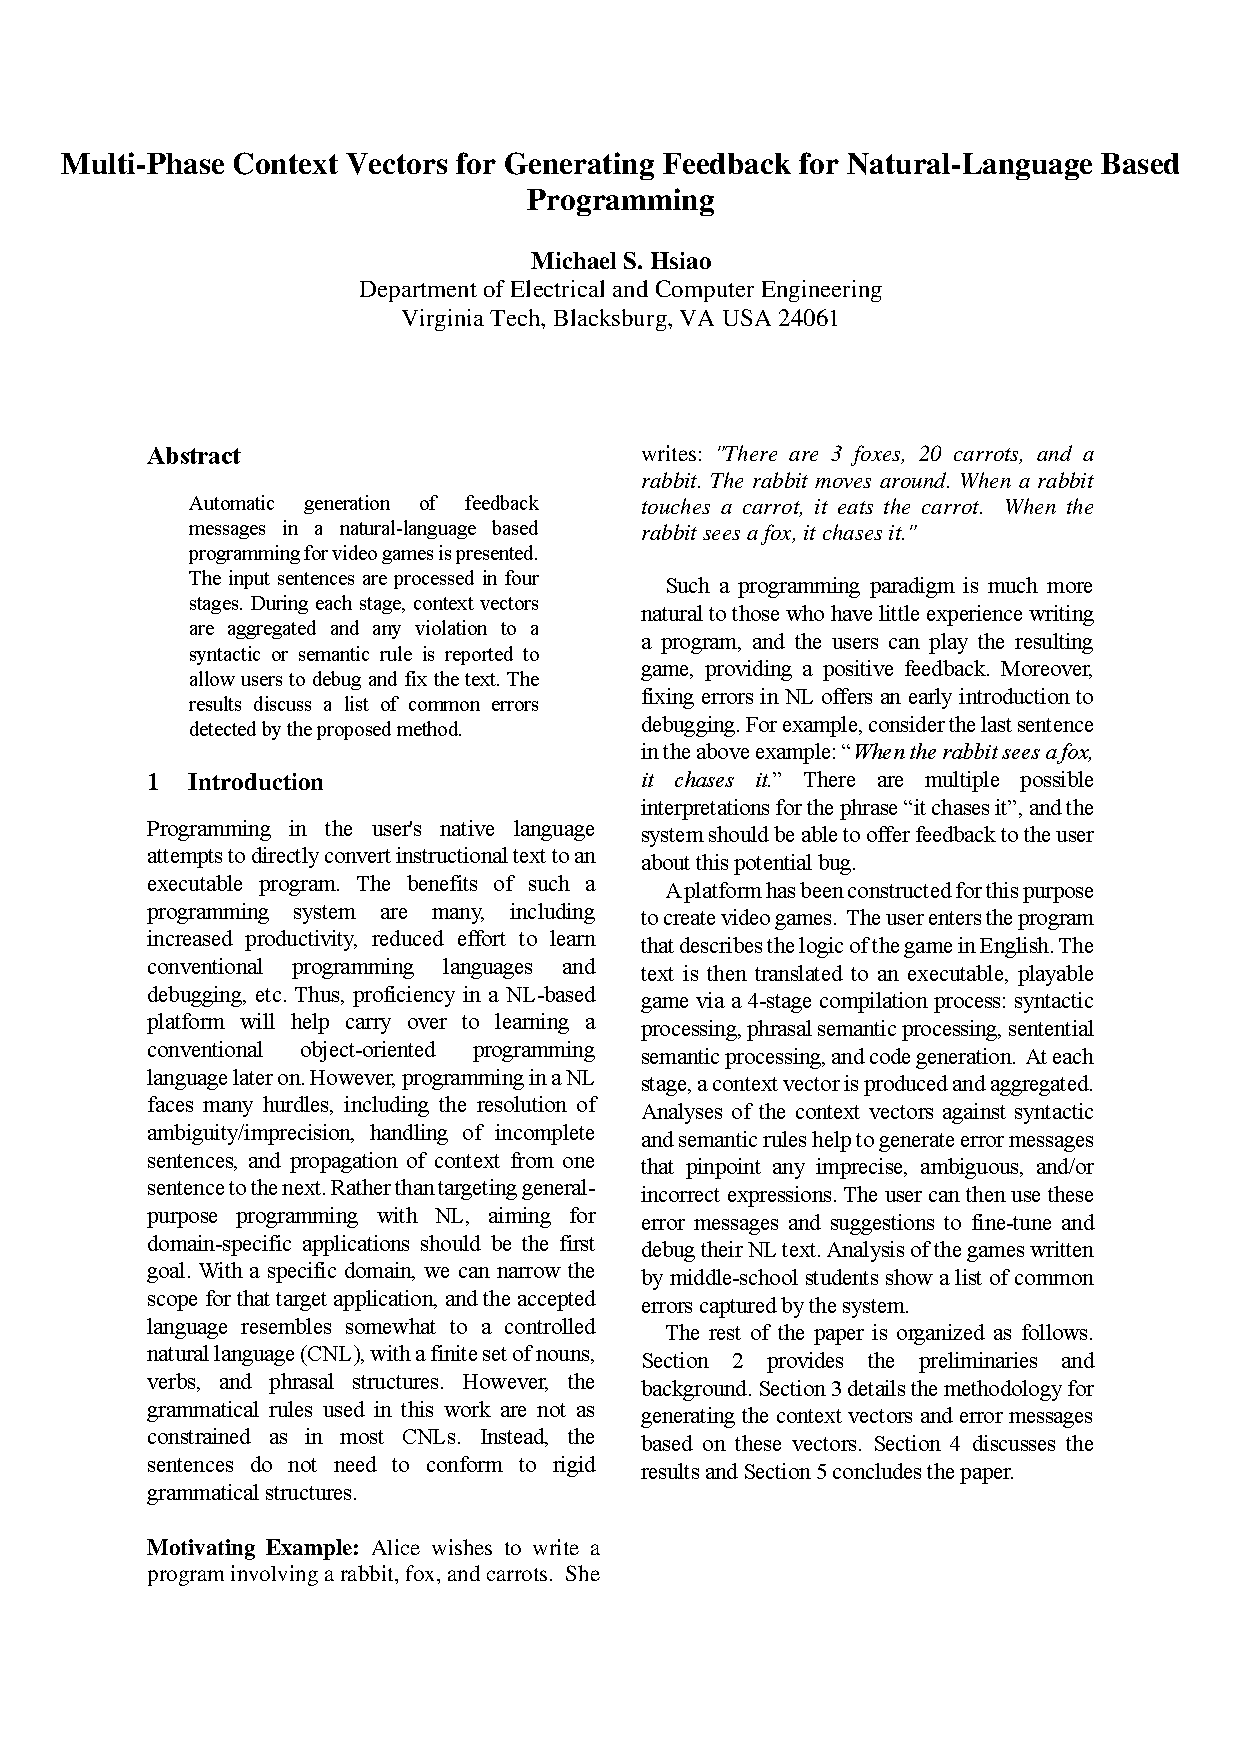
\includepdf[pages=-,pagecommand={}]{../cdrom/pdf/2021.cnl-1.16.pdf}



   % automatically generated from DB file

% -------- END MATTER: AUTHOR INDEX --------

%\ifthenelse{\equal{\draftflag}{1}}{}{
%  \ifthenelse{\isodd{\value{page}}}{}
%    {\newpage \thispagestyle{empty} \phantom{.}}
%  \pagestyle{empty}
%  \printindex
%}

\end{document}
